\subsection{Detaillierte Vegetationsstruktur}


\subsubsection{Vitte, dicht bewachsener Standort}

\begin{figure}[!htb]
        \centering
        \begin{subfigure}[htb]{0.45\textwidth}
                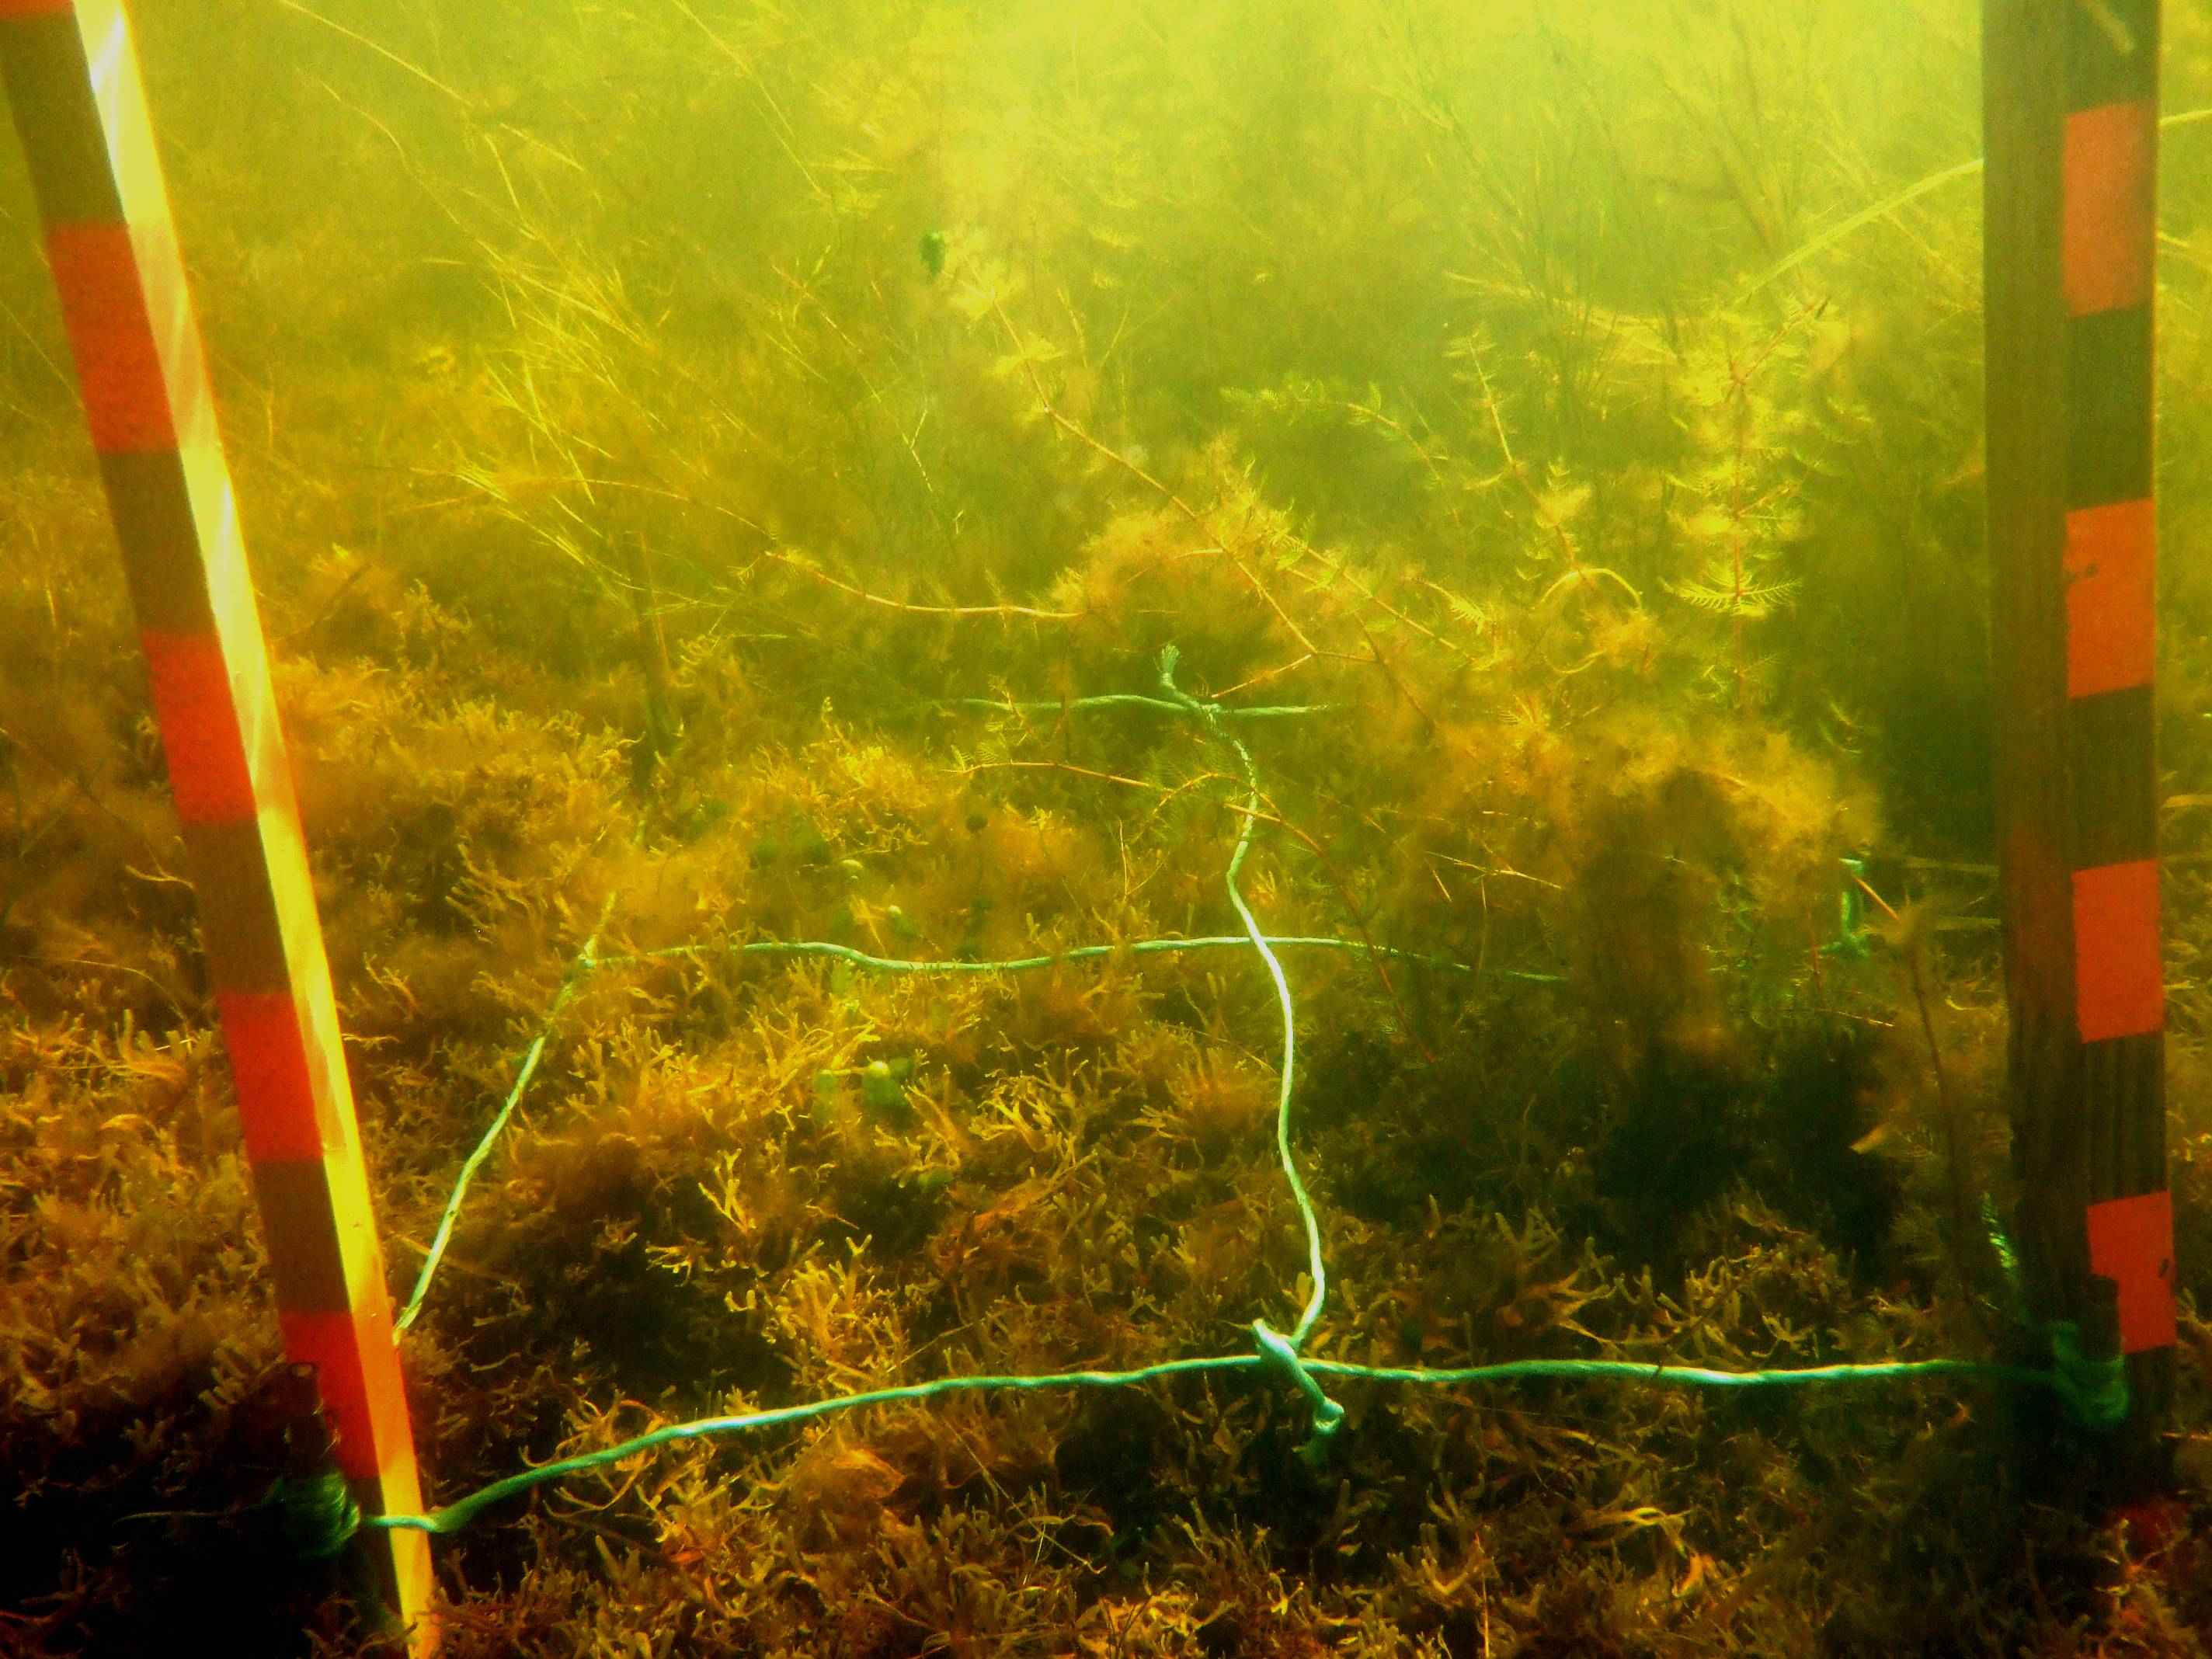
\includegraphics[width=\textwidth]{images/plotpictures/BSP_V+M}
        \end{subfigure}
        \begin{subfigure}[htb]{0.45\textwidth}
                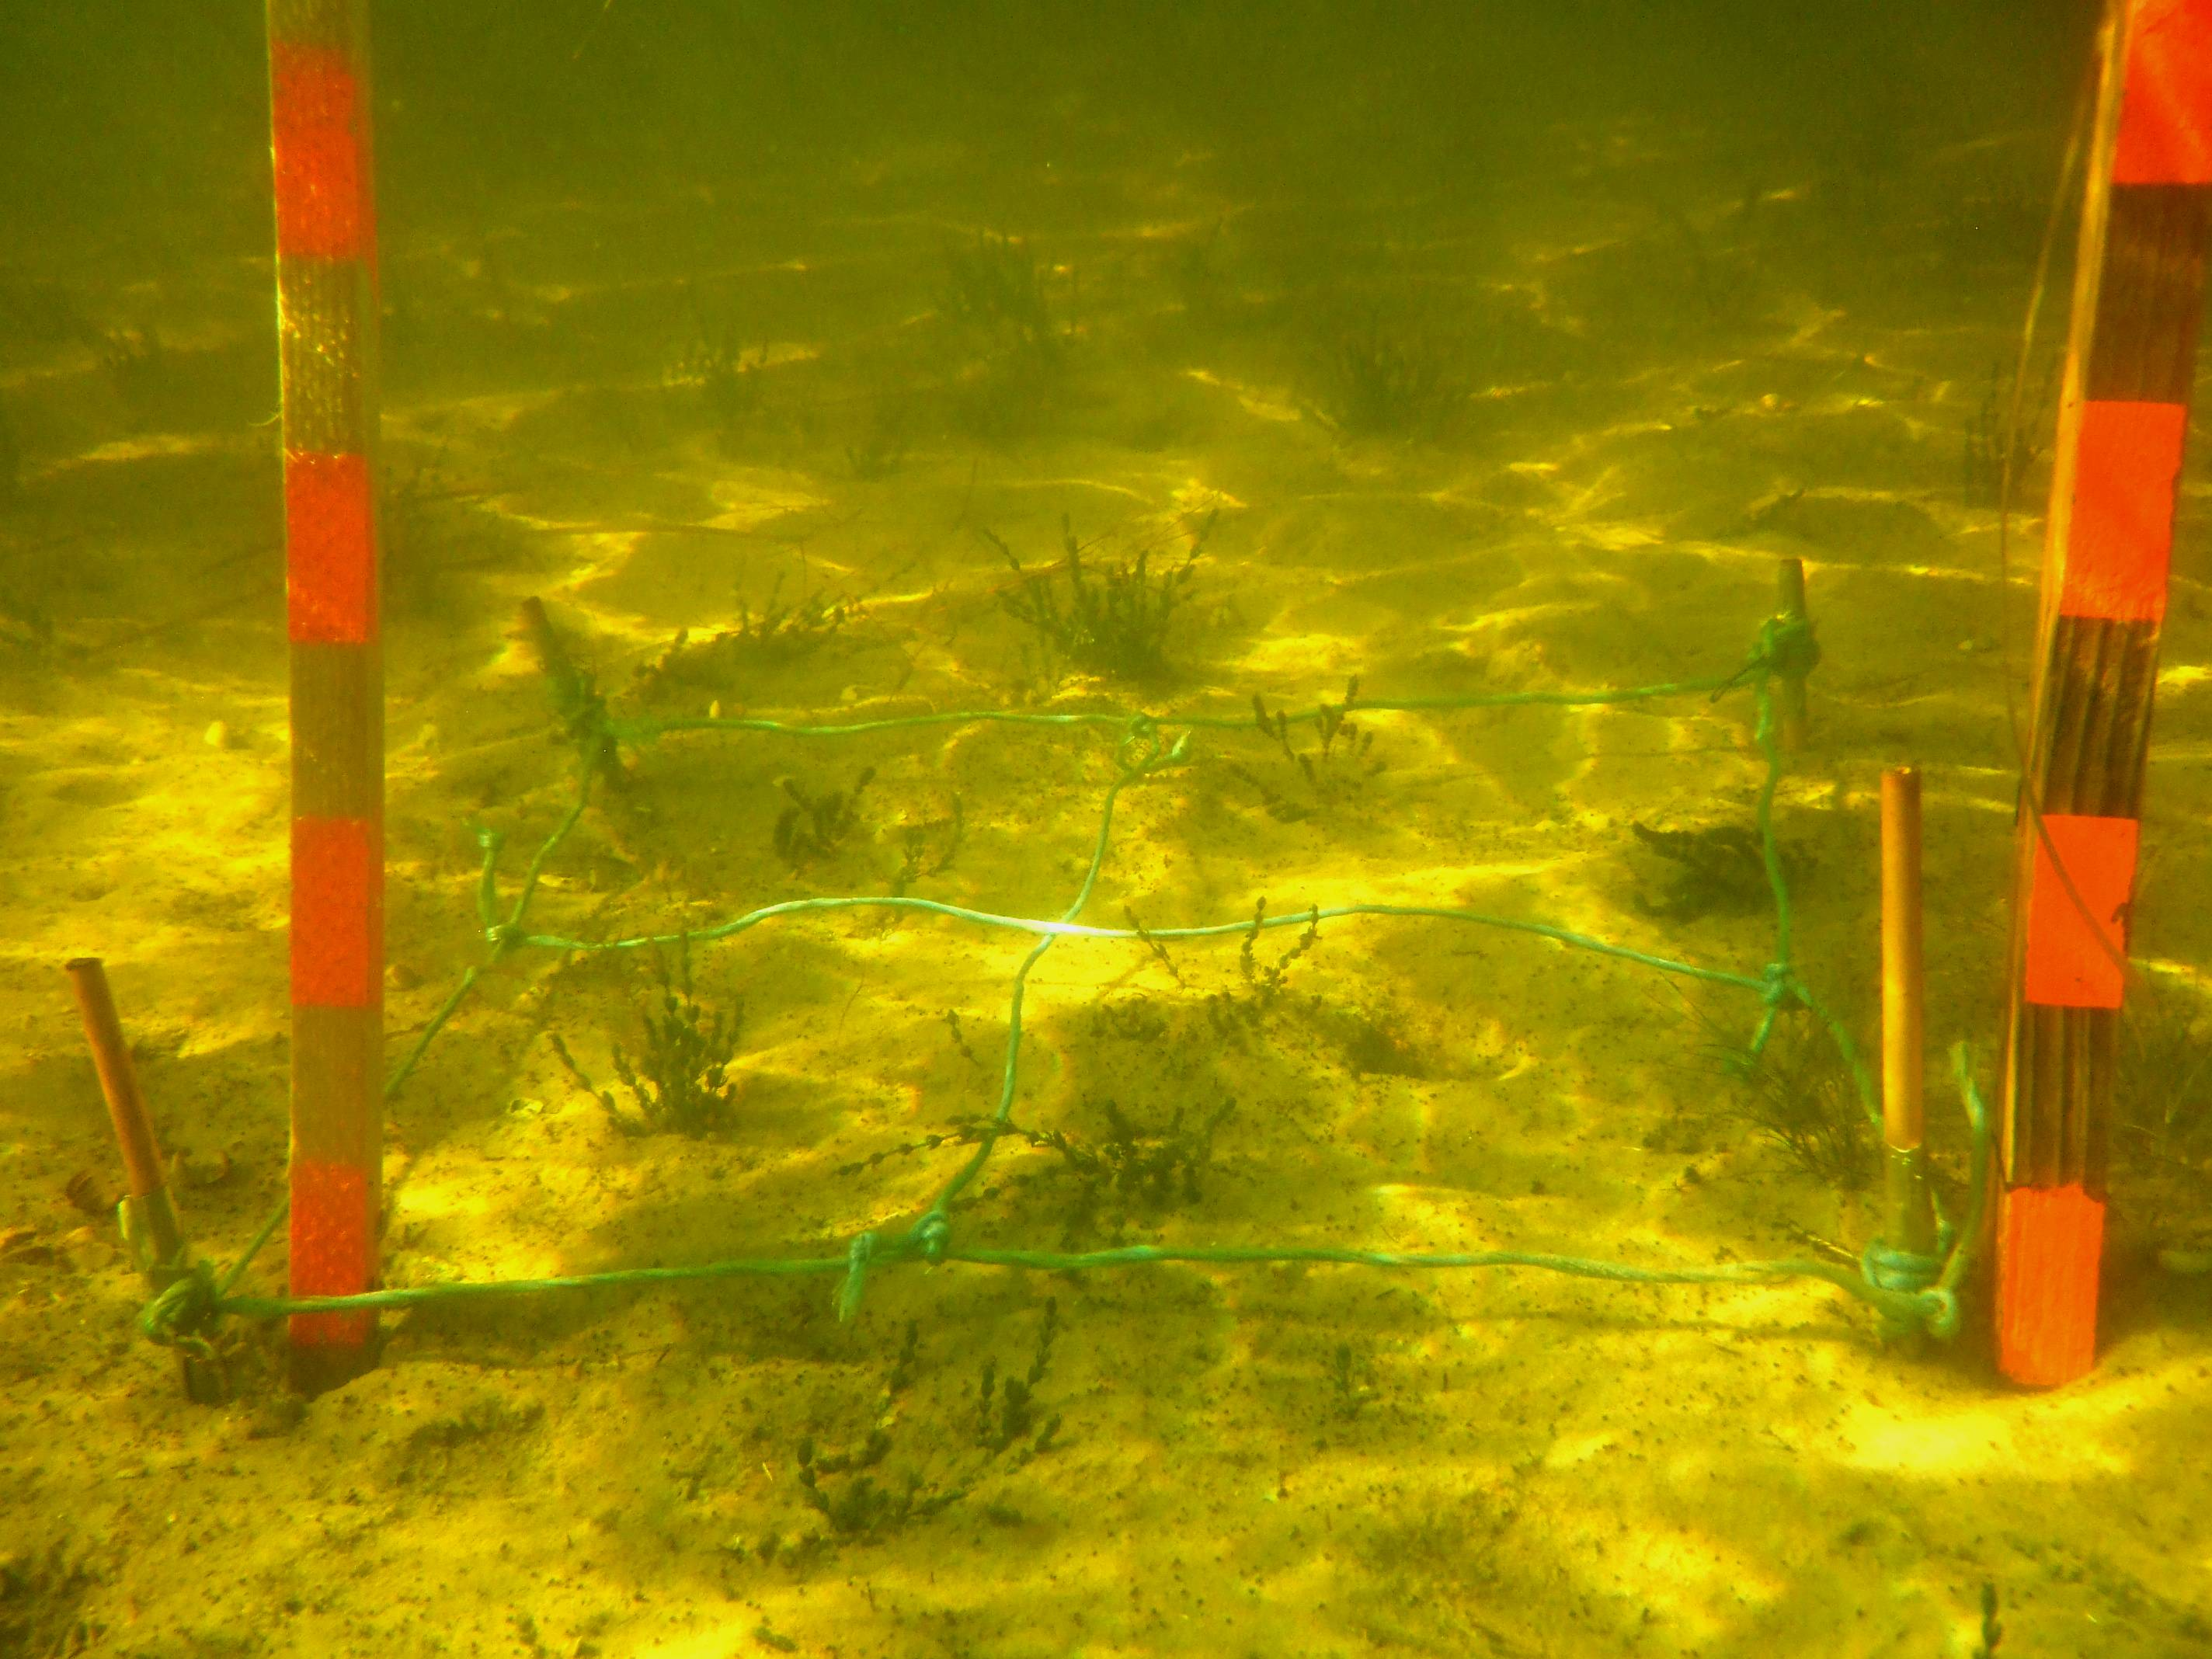
\includegraphics[width=\textwidth]{images/plotpictures/Bsp_V-M}
        \end{subfigure}
        \caption[Fotoaufnahmen der Vegetation in Vitte]{Vegetation in Vitte, vegetationsdominierter Standort 					(links) und  vegetationsarmer Standort (rechts), \unit{0,25}{\metre\squared}- Miniplots, 						Aufnahme August 2013}
        \label{fig:fotos_vitte}
\end{figure}


Die Deckung in Vitte an den vegetationsdominierten Standorten betrug ganzjährig \unit{100}{\%}, wobei der baltische Blasentang \textit{Fucus vesiculosus f. balticus} den Boden vollständig abdeckte. Zwischen dem baltischen Blasentang kam vereinzelt die ebenfalls nicht verwurzelte, kugelförmige Rotalge \textit{Furcellaria fastigiata f. aegagropila} mit einer Deckung von \unit{0,5}{\%} während des gesamten Beobachtungszeitraumes vor. Während die sessilen Makroalgen im Juni bis maximal \unit{5}{\centi\metre}- Wuchshöhe kartiert wurden, sind sie in der Hauptvegetationsperiode (Anfang Juli bis Mitte August) auch auf \unit{10}{\centi\metre} Wuchshöhe mit einer Deckung von \unit{50}{\%} zu finden. Im weiteren Jahresverlauf nimmt die Deckung von \textit{Fucus vesiculosus f. balticus} auf \unit{10}{\centi\metre} Wuchshöhe allmählich wieder ab. Ende August waren es \unit{40}{\%} und Ende September \unit{30}{\%}.

Desweiteren ist die Angiosperme \textit{Potamogeton pectinatus} prägend für den Vitter makrophytendominierten Standort. Mit einer Deckung von \unit{5}{\%} im Mai bis \unit{20}{\%} im August findet sie sich an vielen Stellen zwischen dem dichten Makroalgenteppich und wächst bis an die Wasseroberfläche, an der sich ihr langgestreckter, fadenartiger Wuchs fortsetzt. Insgesamt nimmt die Deckung der Art und die Dichte ihrer Verzweigungen vom Grund zur Oberfläche hin deutlich ab. 

Auch die Angiosperme \textit{Myriophyllum spicatum} findet sich vereinzelt zwischen den Makroalgen mit einer maximalen Deckung von \unit{2}{\%} Ende August. Auch diese zeigt ihre größte Dichte und die meisten Verzweigungen am Grund und nur wenige Äste reichen weiter als \unit{10}{\centi\metre} in den Wasserkörper hinein. Ihre maximale Höhe Ende August beträgt \unit{60}{\centi\metre}.

Im Mai und Juni war der Standort dicht bedeckt von Matten filamentöser Algen, die sich freischwimmend dicht am Grund zwischen den aufwachsenden Angiospermen befanden und später im Jahr verschwanden. Auch die Meerseite \textit{Chorda filum}, eine \unit{40-60}{\centi\metre} lange, fadenförige Braunalge, war im Juni und Juli in alle Plots eingestreut, später im Jahr zog sie sich zusammen und lag schließlich flach eingerollt der \textit{Fucus}-Decke auf. Von Juli bis Ende August wurden zusätzlich Blaualgen-Zellkugeln der Art \textit{Isactis plana} gefunden, die sich vor allem an \textit{Myriophyllum spicatum} und \textit{Potamogeton pectinatus} angeheftet hatten.



\subsubsection{Vitte, spärlich bewachsener Standort}


Dieser Standort war im Juni noch gänzlich unbedeckt. Anfang Juli zeigten sich erste wenige Sprösslinge von \textit{Chara baltica} und \textit{Chara canescens} auf \unit{5}{\centi\metre} Wuchshöhe. Im August wuchs \textit{Chara baltica} bis auf durchschnittlich \unit{10}{\centi\metre}, an einigen Plots auch bis \unit{0,5}{\centi\metre} Deckung auf, während die Bedeckung durch \textit{Chara canescens} unverändert blieb. Zudem traten Anfang August \textit{Potamogeton pectinatus} und \textit{Myriophyllum spicatum} auf einer Wuchshöhe von \unit{5}{\centi\metre} auf, sodass die Gesamtdeckung zu diesem Zeitpunkt \unit{2-5}{\prozent} betrug. \\
Ende August bis Anfang September zeigten sich die höchsten Vegetationsbedeckungen mit \unit{2-20}{\%} bei dieser Untersuchungsgruppe. \textit{Myriophyllum spicatum} und \textit{Potamogeton pectinatus} wuchsen bei gleichbleibend geringer Deckung bis \unit{10}{\centi\metre} auf und \textit{Chara baltica} zeigt nun eine Deckung von \unit{2-5}{\%} auf \unit{10}{\centi\metre}. An einem Plot expantierte \textit{Chara canescens} und bedeckte dort \unit{20}{\%} des Grundes. Auch \textit{Ruppia cirrhosa} trat dazu und bedeckte Ende August zu \unit{0-2}{\%} die Fläche. Im September war \textit{Chara canescens} nicht mehr anwesend, dafür breitete sich \textit{Ruppia cirrhosa} auf den Plots auf einer Höhe von maximal \unit{5}{\centi\metre} mit Deckungsgraden von \unit{0-20}{\%} aus. Auch Seegras (\textit{Zostera marina}) zeigte sich Ende August und Anfang September stellenweise auf den Plots.

\begin{figure}[!htb]
\centering
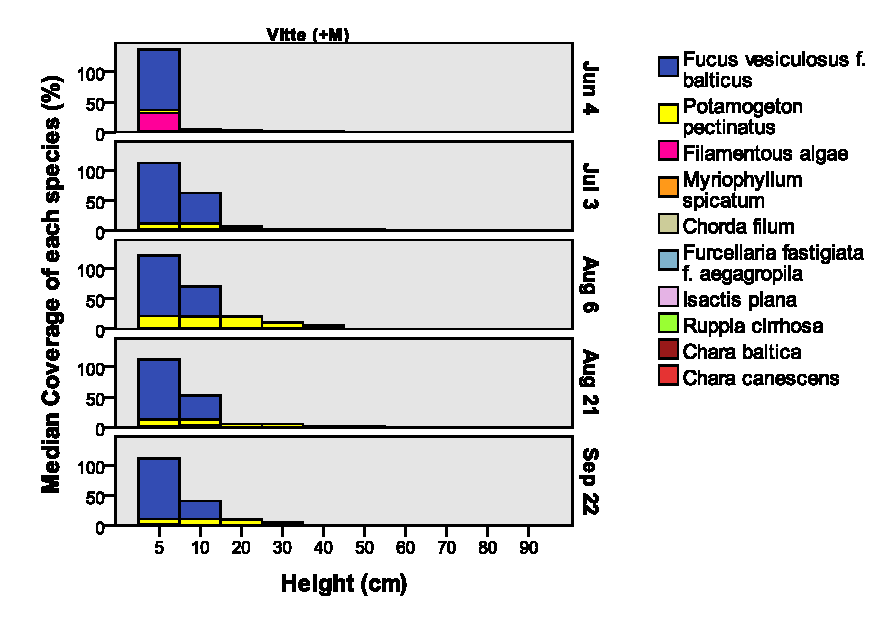
\includegraphics[width=0.90\textwidth]{images/Wuchshoehenkartierung/Vitte+Mb1.eps}
\caption[Höhenstufenkartierung Vitte (+M)]{Deckungen aller Arten auf Höhenstufen vom Grund bis zur Oberfläche, Vitte, dicht bewachsener Standort}
\label{fig:wuchshoehen_vitte_+m1}
\end{figure}
\\
\begin{figure}[!htb]
\centering
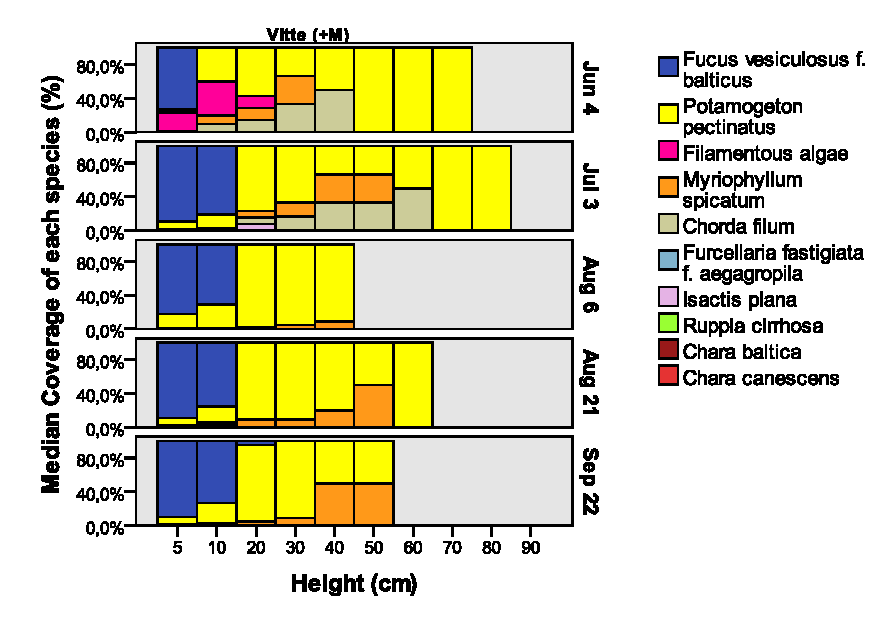
\includegraphics[width=0.90\textwidth]{images/Wuchshoehenkartierung/Vitte+Mb2.eps}
\caption[prozentuale Höhenstufenkartierung Vitte (+M)]{Prozentuale Deckungen aller Arten, bezogen auf die Gesamtdeckung auf jeder Höhenstufe, vom Grund bis zur Oberfläche, Vitte, dicht bewachsener Standort}
\label{fig:wuchshoehen_vitte_+m2}
\end{figure}

\FloatBarrier

\begin{figure}[!htb]
\centering
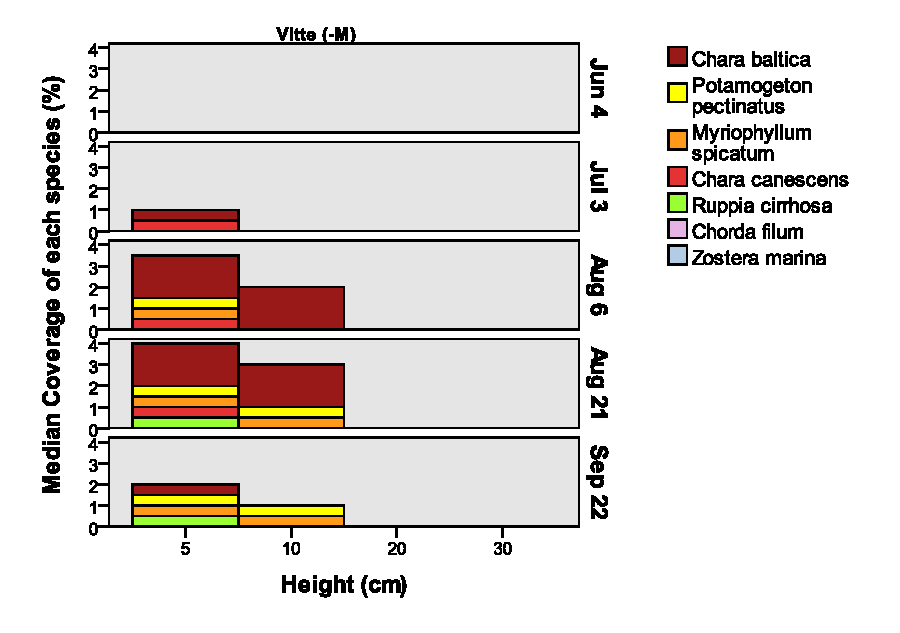
\includegraphics[width=0.90\textwidth]{images/Wuchshoehenkartierung/Vitte-M1.eps}
\caption[Höhenstufenkartierung Vitte (-M)]{Deckungen aller Arten auf Höhenstufen vom Grund bis zur Oberfläche, Vitte, spärlich bewachsener Standort}
\label{fig:wuchshoehen_vitte_-m1}
\end{figure}
\\
\begin{figure}[!htb]
\centering
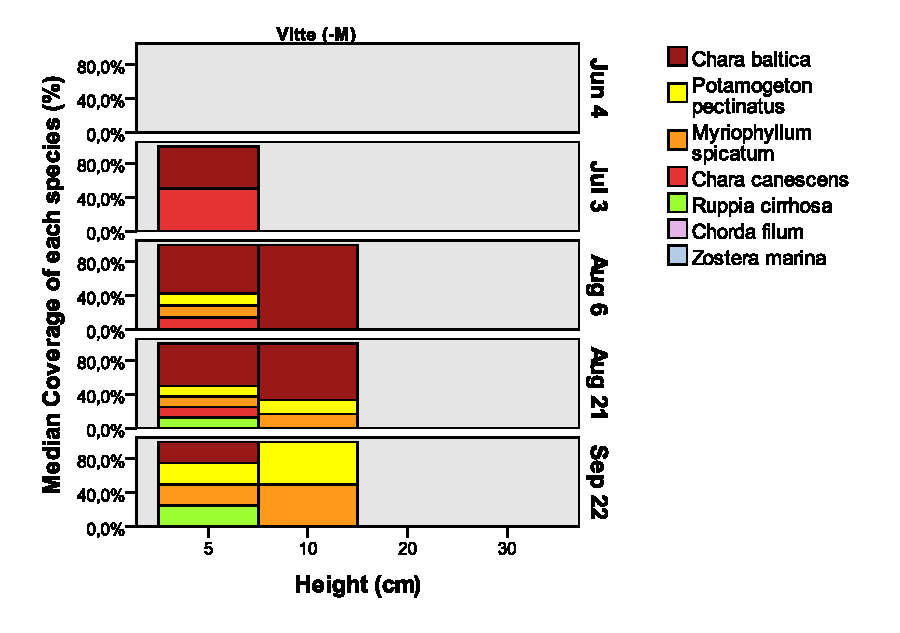
\includegraphics[width=0.90\textwidth]{images/Wuchshoehenkartierung/Vitte-M2.eps}
\caption[prozentuale Höhenstufenkartierung Vitte, vegetationsarmer Standort]{Prozentuale Deckungen aller Arten, bezogen auf die Gesamtdeckung auf jeder Höhenstufe vom Grund bis zur Oberfläche, Vitte, spärlich bewachsener Standort}
\label{fig:wuchshoehen_vitte_-m2}
\end{figure}
\\
\FloatBarrier


\subsubsection{Grieben, dicht bewachsener Standort}


\begin{figure}[!htb]
        \centering
        \begin{subfigure}[htb]{0.45\textwidth}
                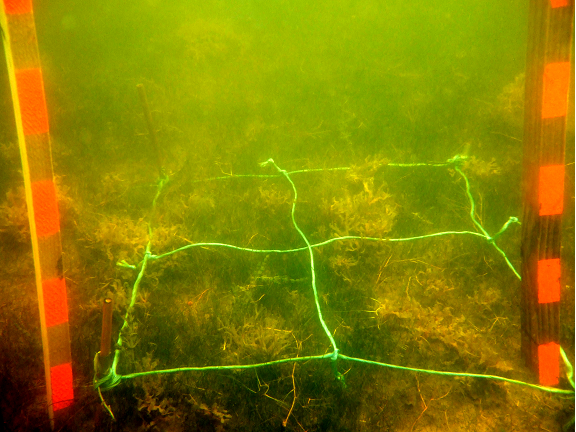
\includegraphics[width=\textwidth]{images/plotpictures/Bsp_G+M}
        \end{subfigure}
        \begin{subfigure}[htb]{0.45\textwidth}
                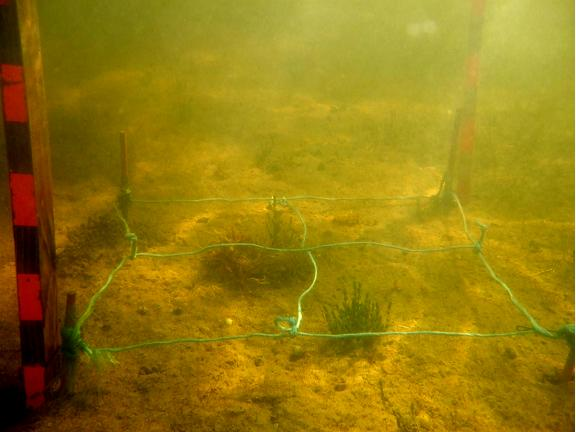
\includegraphics[width=\textwidth]{images/plotpictures/Bsp_G-M}
        \end{subfigure}
        \caption[Fotoaufnahmen der Vegetation in Grieben]{Vegetation in Grieben, vegetationsdominierter 						Standort (links) und  vegetationsarmer Standort (rechts), \unit{0,25}{\metre\squared}- 							Miniplots, Aufnahme August 2013}
        \label{fig:fotos_grieben}
\end{figure}

Die Vegetation am dicht bewachsenen Standort in Grieben ist sehr vielfältig. Im Verlauf der Wachstumssaisong wurden 11 Pflanzenarten kartiert, deren jeweiliges maximales Vorkommen sich abwechselt. Anfang Juni war der Standort zu \unit{30-50}{\%} bedeckt, davon machten ineinander verwobene, fädige Mikroalgen verschiedener Stämme und Arten mit \unit{20-40}{\%} den größten Anteil aus. Sie schwebten lose oder waren zwischen den Makrophyten verhakt. Die dominanten Makrophyten waren \textit{Ruppia cirrhosa} (\unit{10-20}{\%} Deckung) und \textit{Fucus vesiculosus} mit \unit{2-10}{\%} Deckung. An einem Plot war der Anteil von \textit{Fucus vesiculosus} mit \unit{40}{\%} höher. Außerdem wurden jeweils mit geringen Deckungsgraden die Arten \textit{Potamogeton pectinatus} und \textit{Myriophyllum spicatum} sowie \textit{Chara baltica} und \textit{Chorda filum} gefunden. Insgesamt nimmt die Deckung im Juni überhalb \unit{5}{\centri\metre} Höhe vom Grund stark ab. Ab \unit{20}{\centi\metre} Wuchshöhe kommen nur noch \textit{Potamogeton pectinatus} und die fadenförmige Alge \textit{Chorda filum} mit jeweiligen Deckungen unter einem Prozent vor.

Im Juli ging der Anteil filamentöser Algen stark zurück. Sie wurden ans Ufer gespült und starben dort ab. Die Bestände wurden nun hauptsächlich durch die rasig wachsende schraubige Salde \textit{Ruppia cirrhosa} (im Mittel \unit{40}{\%}Deckung)und durch \textit{Potamogeton pectinatus} (\unit{10-30}{\%} Deckung) gebildet. Während \textit{Ruppia cirrhosa} auf \unit{5}{\centi\metre}-Wuchshöhe beschränkt bleibt, ist \textit{Potamogeton pectinatus} deutlich aufgewachsen. Die Pflanzen verzweigen sich im unteren Bereich am Grund und das Volumen nimmt zur Oberfläche hin ab. Auf \unit{10 und 20} {\centi\metre} deckt \textit{Potamogeton pectinatus} durchschnittlich \unit{10 bzw. 2}{\%} der Fläche ab. Mit bis zu \unit{10}{\%} Deckung und bis zu \unit{20}{\centi\metre} tritt erstmals \textit{Chara horrida} im Juli auf.

Anfang August beträgt die Gesamtdeckung auf den Plots bereits \unit{60 bis 70}{\%}. Mit im Mittel \unit{30}{\%} Deckung hat sich \textit{Fucus vesiculosus f. balticus} ausgebreitet und ist bis auf \unit{30}{\centi\metre} vom Grund aufgewachsen. Er zeigt hier seine maximale Deckung. Auch die Bedeckung durch Characeen hat zugenommen. \textit{Chara baltica}, \textit{Chara horrida} und neu hinzugekommen \textit{Chara canescens} bedecken bis zu \unit{5}{\%} die Plots. Während sich \textit{Chorda filum} bereits zurückzog, erschien \textit{Chaetomorpha linum} neu auf den Flächen. Die losen, tellerartig ineinander verschlungenen fadenförmigen Algen wurden auf die Plots verdriftet. \textit{Myriophyllum spicatum} zeigte bei gleichbleibend geringer Gesamtdeckung von unter einem Prozent ihre maximale Wuchshöhe von bis zu \unit{40}{\centi\metre}.

Bis zum September breitete sich \textit{Ruppia cirrhosa} stark aus und bedeckte etwa \unit{60}{\%} der Flächen. Mit Ausnahme einer Aufnahmefläche, deren Gesamtdeckung sich auf \unit{40}{\%} reduzierte, waren die Flächen im September mit \unit{70-100}{\%} maximal mit Pflanzen bedeckt. Die Art blieb während des gesamten Untersuchungszeitraumes kleinwüchsig, selten über die \unit{5}{\centi\metre} Wuchshöhe hinauswachsend und sie bildete keine Fruchtstände. Auffällig war jedoch, dass sie Turionen ausgebildet hatte.

Die zweite Bestandbildende Art im September mit \unit{2-30}{\%} Deckung war \textit{Fucus vesiculosus}. Im Vergleich zum Juli befindet sich die Vegetation auf \unit{5}{\centi\metre} Wuchshöhe konzentriert, auf \unit{10}{\centi\metre} beträgt die Deckung durch Pflanzen lediglich \unit{5}{\%}. Die Characeen sowie \textit{Myriophyllum spicatum} und \textit{Potamogeton pectinatus} haben sich stark zurückgezogen. Neu erschienen sind Algenbüschel von \textit{Polysiphonia violacea}, die sich losgerissen zwischen den Pflanzen und sowie festgewachsen an der Schnur der Schwimmboje befanden. 



\subsubsection{Grieben, spärlich bewachsener Standort}


Zu Beginn der Felduntersuchungen im Juni waren die Flächen vollkommen vegetationsfrei. Bis zum August hat sich dies geändert: \textit{Fucus-vesiculosus}-Bällchen sind an den Standort gedriftet und verursachen Bedeckungen von \unit{2-10}{\%}. Daneben gibt es spärliche Bestände von \textit{Ruppia cirrhosa}, \textit{Chara canescens} und \textit{Chara baltica} mit jeweils unter einem bis zehn Prozent Deckung. \textit{Myriophyllum spicatum} und \textit{Potamogeton pectinatus} sind mit unter einem Prozent Deckung vertreten und wachsen am Höchsten (bis \unit{20}{\centi\metre}) auf. Im Mittel ist der Standort Anfang August zu \unit{5}{\%} mit Pflanzen bedeckt.

Die Vegetationsbedeckung nimmt im weiteren Jahresverlauf zu. Im September wurde die maximale Bedeckung von im Mittel \unit{30}{\%} beobachtet. Maximale und minimale Bedeckungen auf den Plots betrugen \unit{60 bzw. 10}{\%}. Der Anstieg des Anteils der Vegetation wird durch \textit{Fucus vesiculosus f. filiformis }verursacht, der vermehrt auf den Standort verdriftet wurde.\\



\begin{figure}[!htb]
\centering
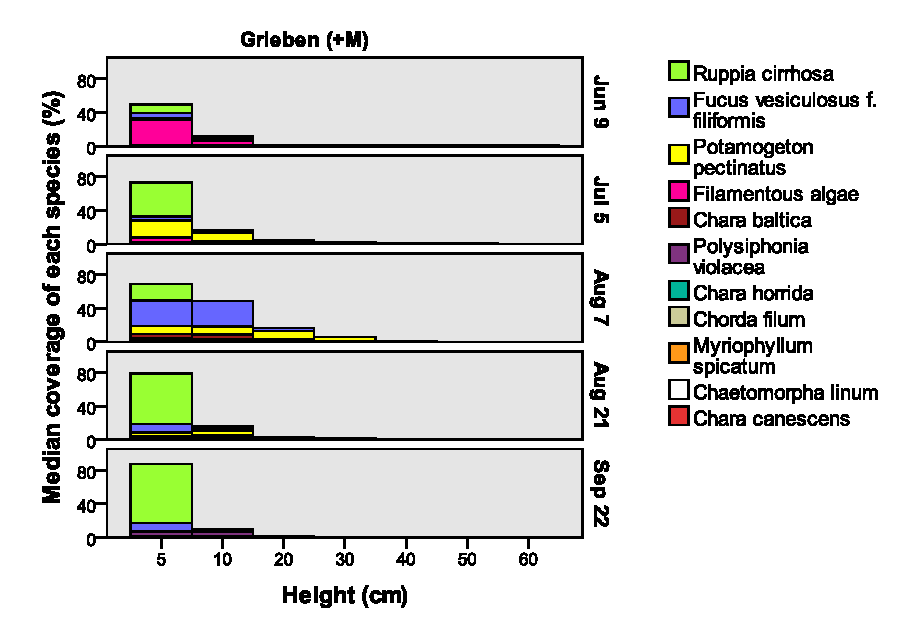
\includegraphics[width=0.90\textwidth]{images/Wuchshoehenkartierung/Grieben+M1.eps}
\caption[Höhenstufenkartierung Grieben (+M)]{Deckungen aller Arten auf Höhenstufen vom Grund bis zur Oberfläche, Grieben, dicht bewachsener Standort}
\label{fig:wuchshoehen_grieben_+m1}
\end{figure}
\\
\begin{figure}[!htb]
\centering
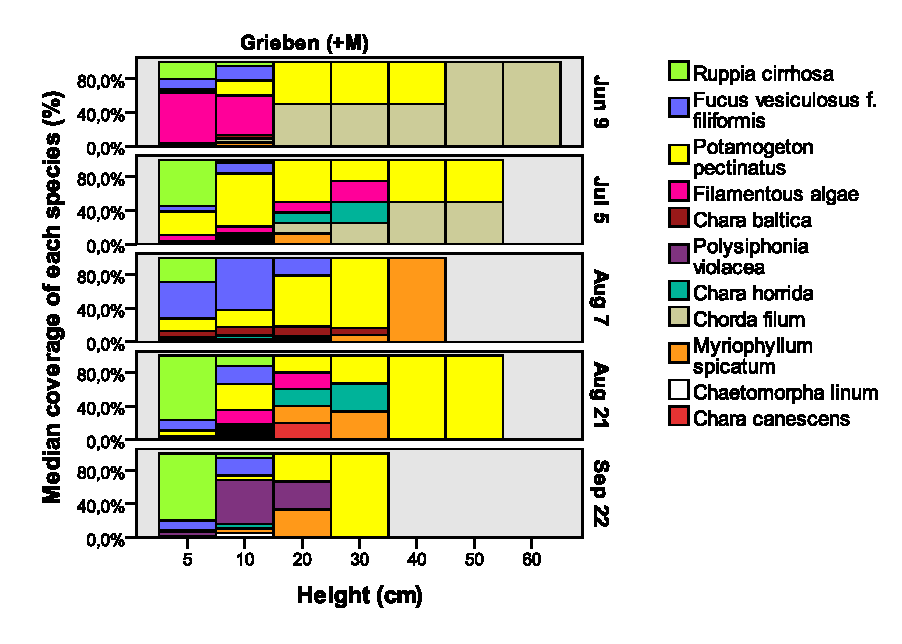
\includegraphics[width=0.90\textwidth]{images/Wuchshoehenkartierung/Grieben+M2.eps}
\caption[prozentuale Höhenstufenkartierung Grieben (+M)]{Prozentuale Deckungen aller Arten, bezogen auf die Gesamtdeckung auf jeder Höhenstufe, vom Grund bis zur Oberfläche, Grieben, dicht bewachsener Standort}
\label{fig:wuchshoehen_grieben_+m2}
\end{figure}

\FloatBarrier

\begin{figure}[!htb]
\centering
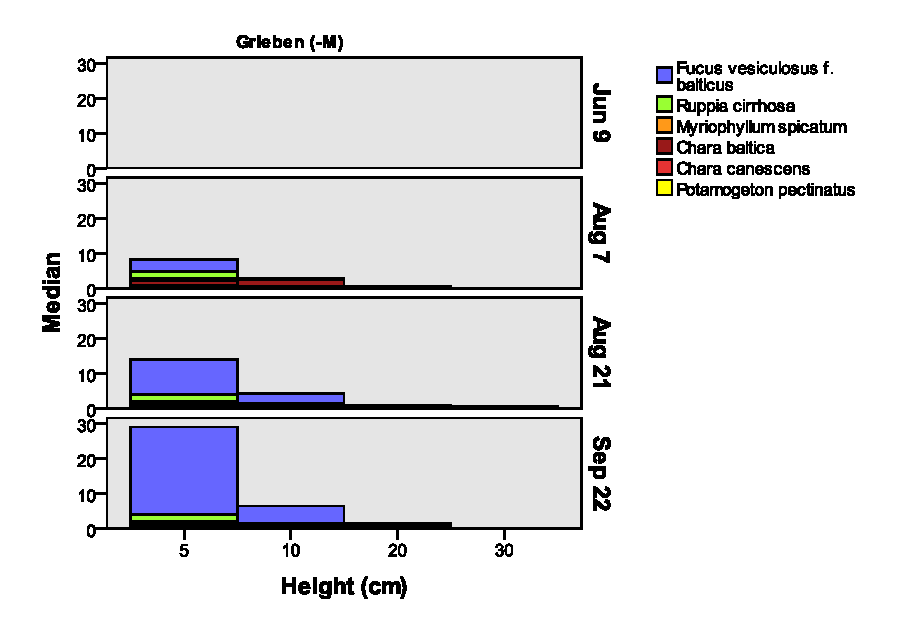
\includegraphics[width=0.90\textwidth]{images/Wuchshoehenkartierung/Grieben-M1.eps}
\caption[Höhenstufenkartierung Grieben (-M)]{Deckungen aller Arten auf Höhenstufen vom Grund bis zur Oberfläche, Grieben, spärlich bewachsener Standort}
\label{fig:wuchshoehen_grieben_-m1}
\end{figure}
\\
\begin{figure}[!htb]
\centering
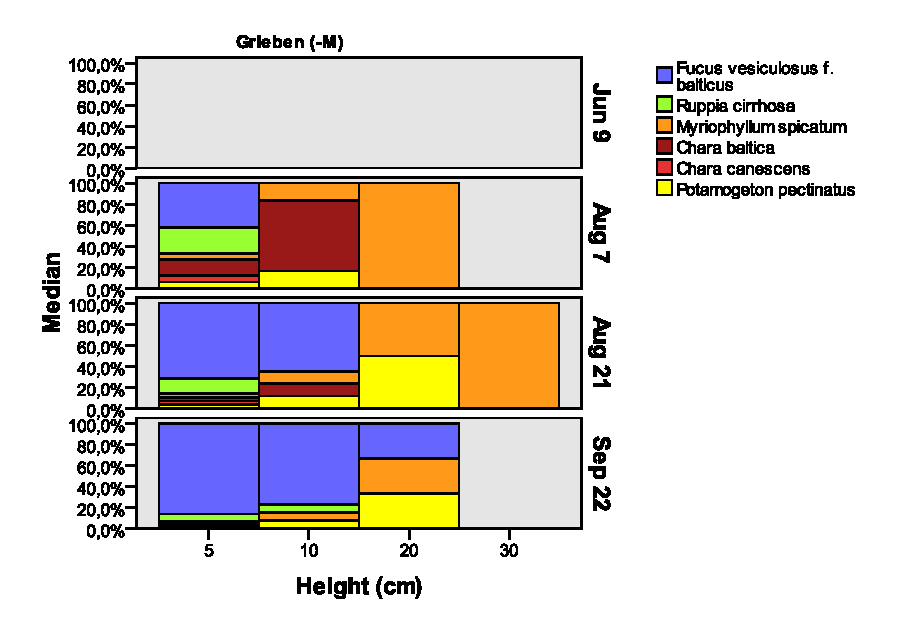
\includegraphics[width=0.90\textwidth]{images/Wuchshoehenkartierung/Grieben-M2.eps}
\caption[prozentuale Höhenstufenkartierung Grieben (-M)]{Prozentuale Deckungen aller Arten, bezogen auf die Gesamtdeckung auf jeder Höhenstufe, vom Grund bis zur Oberfläche, Grieben, spärlich bewachsener Standort}
\label{fig:wuchshoehen_grieben_-m2}
\end{figure}


\FloatBarrier


\subsection{Deckung und PVI}

Sowohl im Vitter Bodden als auch in der Griebener Bucht gab es ganzjährig einen Unterschied in der Bedeckung mit Phytobenthos zwischen den zu Beginn der Vegetationsperiode dicht und spärlich besiedelten Standorten.\\
Im Vitter Bodden war der Unterschied im Juni besonders groß. Die Plots waren vollständig bedeckt beziehungsweise komplett vegetationsfrei. Am vegetationsdominierten Standort verändert sich die Deckung im Jahresverlauf nicht, nur einmal im Juli ist aufgrund eines Ankerwurfes ein Loch in der \textit{Fucus vesiculosus}- dominierten Vegetationsdecke entstanden. Anfang August hatte sich die Decke durch den beweglichen \textit{Fucus} wieder geschlossen.
In der zu Beginn der Studie unbesiedelten Kontrollgruppe im Vitter Bodden hat sich bis Anfang August eine spärliche Vegetationsdecke mit einer mittleren Deckung von \unit{5}{\%} herausgebildet, welche sich bis Ende September aufrecht erhielt.

In der Griebener Bucht war der Unterschied in der Bedeckung zwischen den beiden Untersuchungsgruppen zu Beginn der Studie nicht so groß wie im Vitter Bodden. Die Gruppe auf der Ostseite der Bucht war im Juni vegetationsfrei und die andere zu \unit{30-40}{\%} mit Phytobenthos bedeckt. An beiden Standorten erhöhte sich die Deckung signifikant im Verlauf der Wachstumsperiode. Der dicht besiedelte Bereich war bereits im Juli zu \unit{60}{\%} mit Makrophyten bedeckt, bis Ende September stieg die Deckung allmählich auf \unit{90}{\%} an. Auf dem vorerst nicht besiedelten Bereich entwickelte sich bis Anfang August eine Bedeckung von \unit{5}{\%}. Bis Ende September stieg die Bedeckung auf \unit{30}{\%} an.

Nicht nur die Bedeckung mit Phytobenthos verändert sich im Jahresverlauf, sondern auch dessen Anteil an der Wassersäule. Neben der Wassertiefe, die als mehrjähriger Mittelwert in die Berechnung eingeht, nimmt die zunehmende Wuchshöhe einen Einfluss auf das PVI.

Obwohl das Wasser im Vitter Bodden im dicht besiedelten Bereich mit \unit{83}{\centi\metre} vergleichsweise tief ist, fanden sich hier deutlich höhere Anteile an Makrophytn in der Wassersäule. Im Juni waren es im Mittel \unit{7,7}{\%}. Bis Anfang August stieg der Anteil auf über \unit{15}{\%}. Der spärlich besiedelte Bereich ist mit \unit{62}{\centi\metre} flacher als der dicht besiedelte. Aufgrund der geringen Deckung und der geringen Wuchshöhe betrug das maximale PVI im August und im September \unit{0,6}{\%}. 

In der Griebener Bucht steigt das PVI im Verlauf der Wachstumssaisong in beiden Untersuchungsgruppen deutlich. Bei einer Wassertiefe von \unit{87}{\centi\metre} betrug der Anteil im dicht besiedelten Bereich im Juni \unit{2,4}{\%}. Anfang August erhöhte sich der Anteil auf \unit{7,1}{\%}. Bis zum September nimm das PVI leicht ab, jedoch bewegt sich diese Abnahme auf \unit{5,5}{\%} außerhalb des signifikanten Bereiches.
Der Spärlich besiedelte Bereich ist mit einer durchschnittlichen Tiefe von \unit{65}{\centi\metre} deutlich flacher als der dichtbesiedelte Bereich. Das PVI steigt hier im Verlauf der Wachstumssaisong auf \unit{1,2}{\%} im September an. Ende September gibt es keinen signifikanten Unterschied mehr zwischen dem PVI des dicht und des spärlich besiedelten Bereiches.


\begin{figure}[!htb]
\centering
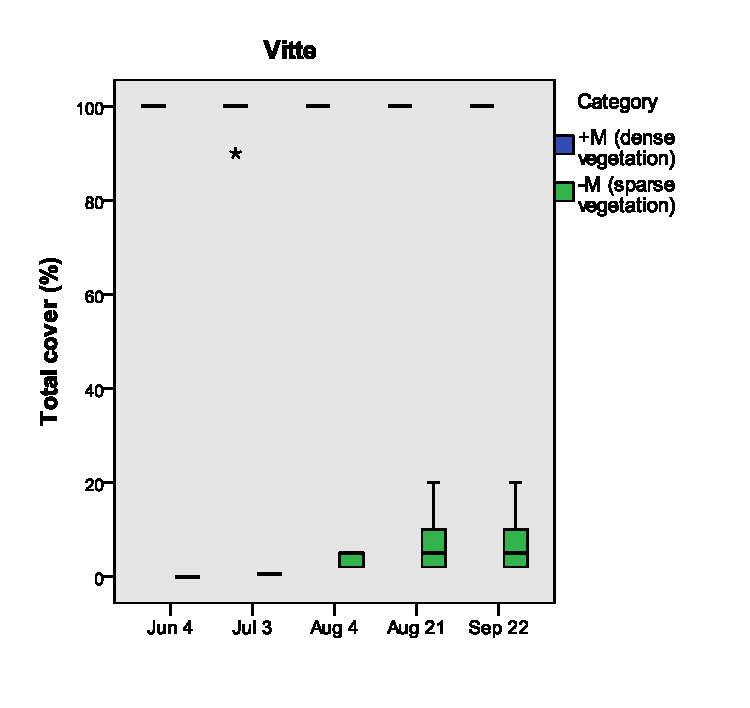
\includegraphics[width=0.70\textwidth]{images/total_cover/Boxplots_G_V1.eps}
\caption[Bedeckung mit Makrophyten, Vitte]{Bedeckung der Hauptuntersuchungs-Plots (\unit{4}{\metre\squared} im Vitter Bodden im Verlauf der Wachstumssaisong 2013}
\label{fig:cover_vitte}
\end{figure}

\begin{figure}[!htb]
\centering
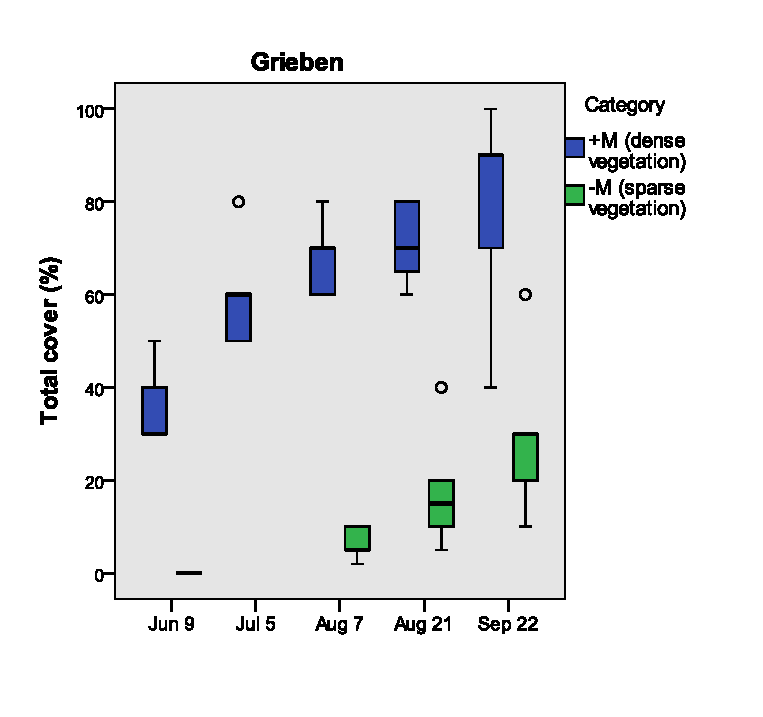
\includegraphics[width=0.70\textwidth]{images/total_cover/Boxplots_G_V2.eps}
\caption[Bedeckung mit Makrophyten, Grieben]{Bedeckung der Hauptuntersuchungs-Plots (\unit{4}{\metre\squared} in der Griebener Bucht im Verlauf der Wachstumssaisong 2013}
\label{fig:cover_grieben}
\end{figure}



\begin{figure}[!htb]
\centering
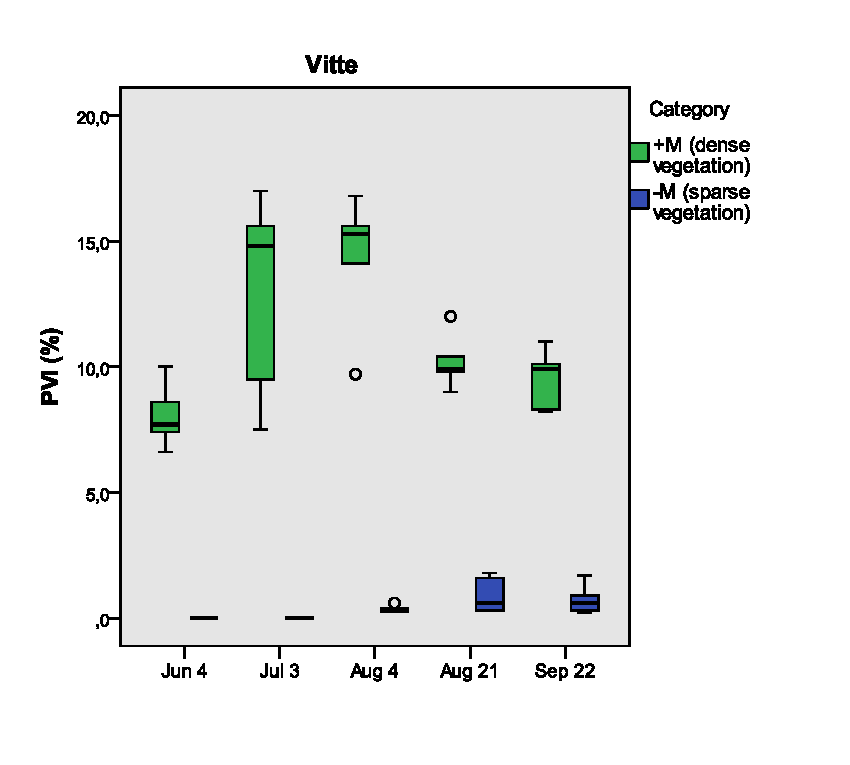
\includegraphics[width=0.70\textwidth]{images/pvi/boxplot_pvi1.eps}
\caption[PVI, Vitte]{Anteil des Phytobenthos an der Wassersäule (PVI nach \cite{jeppesen_1998}) im Vitter Bodden im Verlauf der Wachstumssaisong 2013}
\label{fig:pvi_vitte}
\end{figure}

\begin{figure}[!htb]
\centering
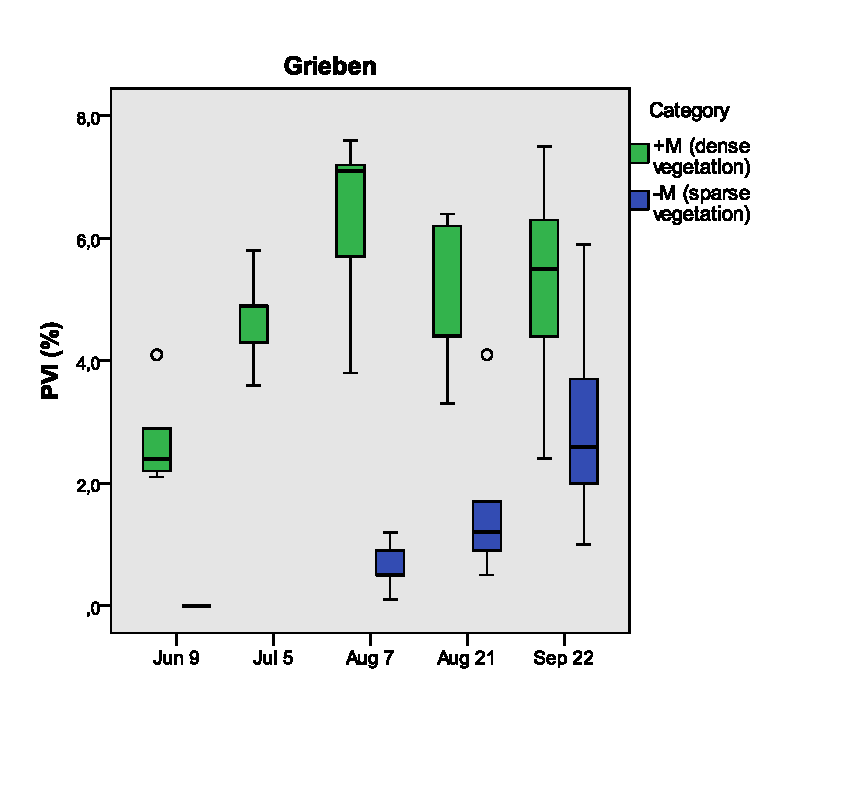
\includegraphics[width=0.70\textwidth]{images/pvi/boxplot_pvi2.eps}
\caption[PVI, Grieben]{Anteil des Phytobenthos an der Wassersäule (PVI nach \cite{jeppesen_1998}) in der Griebener Bucht im Verlauf der Wachstumssaisong 2013}
\label{fig:pvi_grieben}
\end{figure}

\FloatBarrier




\begin{table}[!htb]{\textwidth}
\centering
\caption[Teststatistik Unterschiede zwischen -M und +M in Grieben und Vitte]{Mann-Whithney-Teststatistik zur Ermittlung von Unterschieden in Deckung und PVI zwischen dicht und spärlich mit Phytobenthos besiedelten Standorten im Vitter Bodden und in der Griebener Bucht}
\begin{tabular}{lrrrrrr}
\toprule

Location					& Date		& \multicolumn{2}{c}{Total Cover} 	& \multicolumn{2}{c}{PVI}\\
\midrule
							&	& \multicolumn{1}{c}{Z} & \multicolumn{1}{c}{\textit{p}}& \multicolumn{1}{c}{Z}	& \multicolumn{1}{c}{\textit{p}}\\
\midrule
\multirow{5}{*}{Vitter Bodden}& Jun 04 	& -3.000 		& 0.008\ast			& -2.785			& 0.008\ast\\
 							& Jul 03    & -2.887	    & 0.008\ast 		& -2.783			& 0.008\ast\\
							& Aug 04	& -2.835		& 0.008\ast	     	& -2.643 			& 0.008\ast\\
							& Aug 21	& -2.798 		& 0.008\ast		    & -2.619			& 0.008\ast\\
							& Sep 22	& -2.795 		& 0.008\ast			& -2.611			& 0.008\ast\\
\midrule
\multirow{5}{*}{Griebener Bucht}& Jun 09& -2.825		& 0.008\ast		    & -2.785		& 0.008\ast\\
							& Aug 07	& -2.643		& 0.008\ast		    & -2.619		& 0.008\ast\\
							& Aug 21	& -2.619		& 0.008\ast		    & -2.410		& 0.016\ast\\
							& Sep 22	& -2.417		& 0.016\ast		    & -1.567		& 0.151\\
							
\bottomrule
\end{tabular}
\label{tab:mann_whithney_v,g}
\end{table}



\begin{table}[!htb]{\textwidth}
\centering
\caption[Deskriptive Statistik, Deckung und PVI in Grieben und Vitte]{Deskriptive Statistik zu Deckung und PVI in Vitter Bodden und Griebener Bucht; +M = dichte Vegetation, -M = spärliche Vegetation, MAD = Mittlere Abweichung vom Median}
\begin{tabular}{lrrrrr}
\toprule
Location & \multicolumn{1}{c}{Date}	& \multicolumn{2}{c}{Total Cover} 	& \multicolumn{2}{c}{PVI}\\
\midrule
							&			& Median 		& MAD				& Median		& MAD\\
\midrule
\multirow{5}{*}{Vitter Bodden (+M)} & Jun 04 	& 100.00 		& 0.00				& 7.70			& 0.92\\
 							& Jul 03    & 100.00	    & 2.00				& 14.80			& 3.12\\
							& Aug 04	& 100.00		& 0.00				& 15.30			& 1.72\\
							& Aug 21	& 100.00		& 0.00				& 9.90			& 0.72\\
							& Sep 22	& 100.00		& 0.00				& 9.90			& 0.92\\
\midrule
\multirow{5}{*}{Vitter Bodden (-M)} & Jun 04	& 0.00			& 0.00				& 0.00			& 0.00\\
							& Jul 03	& 0.00			& 0.00				& 0.00			& 0.00\\
							& Aug 06	& 5.00			& 1.20				& 0.30			& 0.08\\
							& Aug 21	& 5.00			& 5.20				& 0.60			& 0.56\\
							& Sep 22	& 5.00			& 5.20				& 0.60			& 0.42\\
\midrule
\multirow{5}{*}{Griebener Bucht (+M)}& Jun 09	& 30.00			& 6.00				& 2.42			& 0.54\\
							& Jul 05	& 60.00			& 8.00				& 4.90			& 0.56\\
							& Aug 07	& 70.00			& 6.00				& 7.10			& 1.06\\
							& Aug 21	& 70.00			& 7.00				& 4.40			& 0.98\\
							& Sep 22	& 90.00			& 16.00				& 5.50			& 1.40\\
\midrule	
\multirow{4}{*}{Griebener Bucht (-M)}& Jun 09	& 0.00			& 0.00				& 0.00			& 0.00\\
							& Aug 07	& 5.00			& 2.60				& 0.50			& 0.30\\
							& Aug 21	& 15.00			& 9.00				& 1.20			& 0.88\\
							& Sep 22	& 30.00			& 12.00				& 2.60			& 1.32\\
\bottomrule
\end{tabular}
\label{tab:statistik_G,V_Deckung,PVI}
\end{table}

\FloatBarrier


\begin{table}[!htb]{\textwidth}
\centering
\caption[Teststatistik Unterschiede in der Deckung im Jahresverlauf in Grieben und Vitte]{Kruskal-Wallis-Teststatistik zur Ermittlung von Unterschieden in der Bedeckung mit Phytobenthos im Jahresverlauf sowie Multiple Vergleiche mit dem Dunn's Test bei Signifikanz (\textit{p} < 0,05; Kennzeichnung mit Stern) im Vitter Bodden und in der Griebener Bucht}
\begin{tabular}{lrcrlr}

\toprule

Location & \multicolumn{3}{c}{Kruskal Wallis Test} 	& \multicolumn{2}{c}{Dunn's Multiple Comparisons Test}\\
\midrule
& \multicolumn{1}{c}{\chi\squared} & df & \multicolumn{1}{c}{\textit{p}-Value} & \multicolumn{1}{c}{Date} & \multicolumn{1}{c}{\textit{p}-Value}\\
&&& (Asymptotic) && \multicolumn{1}{c}{(Adjusted)}\\
\midrule
Vitte (+M)	& 4.000 & 4 & 0.406 \\
\midrule
\multirow{10}{*}{Vitter Bodden (-M)}	& 19.384 & 4 & 0.001\ast & Jun 4 vs. Jul 03 & > 0.999\\
														&&&& Jun 04 vs. Aug 06 & 0.025\ast\\
														&&&& Jun 04 vs. Aug 21& 0.006\ast\\
														&&&& Jun 04 vs. Sep 22&	0.006\ast\\
														&&&& Jul 03 vs. Aug 06&	0.540\\
														&&&& Jul 03 vs. Aug 21&	0.203\\
														&&&& Jul 03 vs. Sep 22&	0.203\\
														&&&& Aug 06 vs. Aug 21&	> 0.999\\
														&&&& Aug 06 vs. Sep 22&	> 0.999\\
														&&&& Aug 21 vs. Sep 22&	> 0.999\\
\midrule
\multirow{10}{*}{Griebener Bucht (+M)} & 13.283 & 4 & 0.010\ast & Jun 09 vs. Jul 05 & 0.906\\
															&&&& Jun 09 vs. Aug 07 & 0.119\\
															&&&& Jun 09 vs. Aug 21 & 0.048\ast\\
															&&&& Jun 09 vs. Sep 22 & 0.001\ast\\
															&&&& Jul 05 vs. Aug 07 & > 0.999\\
															&&&& Jul 05 vs. Sep 22 & > 0.999\\
															&&&& Aug 07 vs. Aug 21 & > 0.999\\
															&&&& Aug 07 vs. Sep 22 & > 0.999\\
															&&&& Aug 21 vs. Sep 22 & > 0.999\\
\midrule
\multirow{6}{*}{Griebener Bucht (-M)} & 15.112 & 3 & 0.002\ast & Jun 09 vs. Aug 07	& 	0.624\\
															&&&& Jun 09 vs. Aug 21	&	0.025\ast\\
															&&&& Jun 09 vs. Sep 22	&	0.002\ast\\
															&&&& Aug 07 vs. Aug 21	&	> 0.999\\
															&&&& Aug 07 vs. Sep 22	&	0.270\\
															&&&& Aug 21 vs. Sep 22	&	> 0.999\\
															
\bottomrule
\end{tabular}
\label{tab:kruskal_wallis_deckung_v,g}
\end{table}





\begin{table}[!htb]{\textwidth}
\centering
\caption[Teststatistik: Unterschiede des PVI im Jahresverlauf in Grieben und Vitte]{Kruskal-Wallis-Teststatistik zur Ermittlung von Unterschieden im Anteil des Phytobenthos an der Wassersäule (PVI) sowie Multiple Vergleiche mit dem Dunn's Test bei Signifikanz (\textit{p} < 0,05, Kennzeichnung mit Stern)im Vitter Bodden und in der Griebener Bucht}
\begin{tabular}{lrcrlr}

\toprule

Location & \multicolumn{3}{c}{Kruskal Wallis Test} 	& \multicolumn{2}{c}{Dunn's Multiple Comparisons Test}\\
\midrule
& \multicolumn{1}{c}{\chi\squared} & df & \multicolumn{1}{c}{\textit{p}-Value} & \multicolumn{1}{c}{Date} & \multicolumn{1}{c}{\textit{p}-Value}\\
&&& (Asymptotic) && (Adjusted)\\
\midrule
Vitte (+M)	& 4.000 & 4 & 0.406 \\
\midrule
\multirow{10}{*}{Vitter Bodden (+M)} & 9.836 & 4 & 0.043\ast & Jun 04 vs. Jul 03 & 0.269\\
&&&& Jun 04 vs. Aug 06	&	0.032\ast\\
&&&& Jun 04 vs. Aug 21	&	> 0.999\\
&&&& Jun 04 vs. Sep 22	&	> 0.999\\
&&&& Jul 03 vs. Aug 06	&	> 0.999\\
&&&& Jul 03 vs. Aug 21	&	> 0.999\\
&&&& Jul 03 vs. Sep 22	&	> 0.999\\
&&&& Aug 06 vs. Aug 21	&	> 0.999\\
&&&& Aug 06 vs. Sep 22	&	0.780\\
&&&& Aug 21 vs. Sep 22	&	> 0.999\\													
\midrule
\multirow{10}{*}{Vitter Bodden (-M)} & 19.276 & 4 & 0.025\ast & Jun 04 vs. Jul 03 &	> 0.999\\
&&&& Jun 04 vs. Aug 06	&	0.157\\
&&&& Jun 04 vs. Aug 21	&	0.019\ast\\
&&&& Jun 04 vs. Sep 22	&	0.042\ast\\
&&&& Jul 03 vs. Aug 06	&	0.157\\
&&&& Jul 03 vs. Aug 21	&	0.019\ast\\
&&&& Jul 03 vs. Sep 22	&	0.042\ast\\
&&&& Aug 06 vs. Aug 21	&	> 0.999\\
&&&& Aug 06 vs. Sep 22	&	> 0.999\\
&&&& Aug 21 vs. Sep 22	&	> 0.999\\
\midrule
\multirow{10}{*}{Griebener Bucht (+M)} & 11.164 & 4 & 0.025\ast & Jun 09 vs. Jul 05 & 0.613\\
															&&&& Jun 09 vs. Aug 07 & 0.014\ast\\
															&&&& Jun 09 vs. Aug 21 & 0.332\\
															&&&& Jun 09 vs. Sep 22 & 0.180\\
															&&&& Jul 05 vs. Aug 07 & > 0.999\\
															&&&& Jul 05 vs. Sep 22 & > 0.999\\
															&&&& Aug 07 vs. Aug 21 & > 0.999\\
															&&&& Aug 07 vs. Sep 22 & > 0.999\\
															&&&& Aug 21 vs. Sep 22 & > 0.999\\
\midrule
\multirow{6}{*}{Griebener Bucht (-M)} & 14.926 & 3 & 0.002\ast & Jun 09 vs. Aug 07	& 	0.565\\
															&&&& Jun 09 vs. Aug 21	&	0.035\ast\\
															&&&& Jun 09 vs. Sep 22	&	0.002\ast\\
															&&&& Aug 07 vs. Aug 21	&	> 0.999\\
															&&&& Aug 07 vs. Sep 22	&	0.275\\
															&&&& Aug 21 vs. Sep 22	&	> 0.999\\
															
\bottomrule
\end{tabular}
\label{tab:kruskal_wallis_pvi_v,g}
\end{table}
\\
\\
\\
\\
\\

\FloatBarrier


\subsection{Biomasse}

Bereits Anfang Juli gab es im Vitter Bodden auf den vegetationsdominierten Untersuchungsflächen im Mittel Biomassewerte von \unit{558}{\gram\per\metre\squared} Trockensubstanz. Dabei ist die mittlere Abweichung vom Median recht groß, auf einer Untersuchungsfläche fanden sich sogar etwa \unit{800}{\gram\per\metre\squared}. Bis zum August erhöht sich die Biomasse auf den Plots auf im Mittel \unit{890}{\gram\per\metre\squared}. Es gibt einen deutlichen Unterschied zu der vegetationsarmen Untersuchungsgruppe. Hier gab es im Mittel \unit{15}{\gram\per\metre\squared} Trocken-Biomasse im August. Etwa gleich viel (\unit{16,5}{\gram\per\metre\squared}) fanden sich auch in der Griebener Bucht im spärlich bewachsenen Bereich. 

Auch die Biomasse in der Griebener Bucht unterscheidet sich signifikant zwischen den beiden Untersuchungsgruppen, jedoch waren hier die Biomassewerte im dicht bewachsenen Bereich von im Mittel \unit{132}{\gram\per\metre\squared} im Juli und \unit{126}{\gram\per\metre\squared} im August  deutlich geringer als die des dicht bewachsenen Bereiches im \textit{Fucus vesiculosus }-dominierten Vitter Bodden. Es gab hier keine signifikante Zunahme der Biomasse von Anfang Juli bis Anfang August.

Der Organische Gehalt der Biomasse unterscheidet sich zwischen den Standorten im Vitter Bodden \unit{60-68}{\gram\per\metre\squared} und in der Griebener Bucht \unit{80-81}{\gram\per\metre\squared}. Es gibt jedoch jeweils keine signifikanten Unterschiede zwischen den vegetationsarmen und vegetationsreichen Untersuchungsgruppen.


\begin{figure}[!htb]
\centering
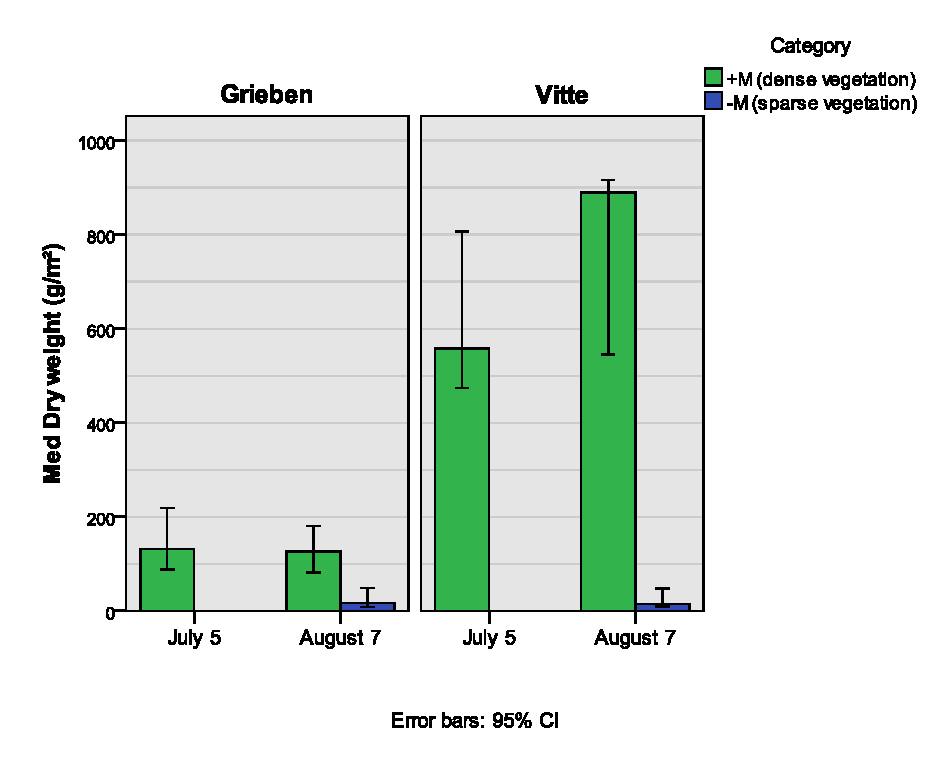
\includegraphics[width=0.80\textwidth]{images/biomass/biomasse_berichtigt1.eps}
\caption[Biomasse an den Hiddenseer Standorten]{Biomasse (Trockengewicht) geerntet auf Miniplots (\unit{0,25}{\metre\squared} neben den Hauptuntersuchungsplots in Grieben und Vitte, Probenahme Anfang Juli (nur dicht bewachsene Standorte) und Anfang August (dicht und spärlich bewachsene Standorte); Median (Balken) und \unit{95}{\%}-Bereich(Antennen) der Daten von jeweils 5 Replikaten}
\label{fig:biomasse}
\end{figure}

\begin{figure}[!htb]
\centering
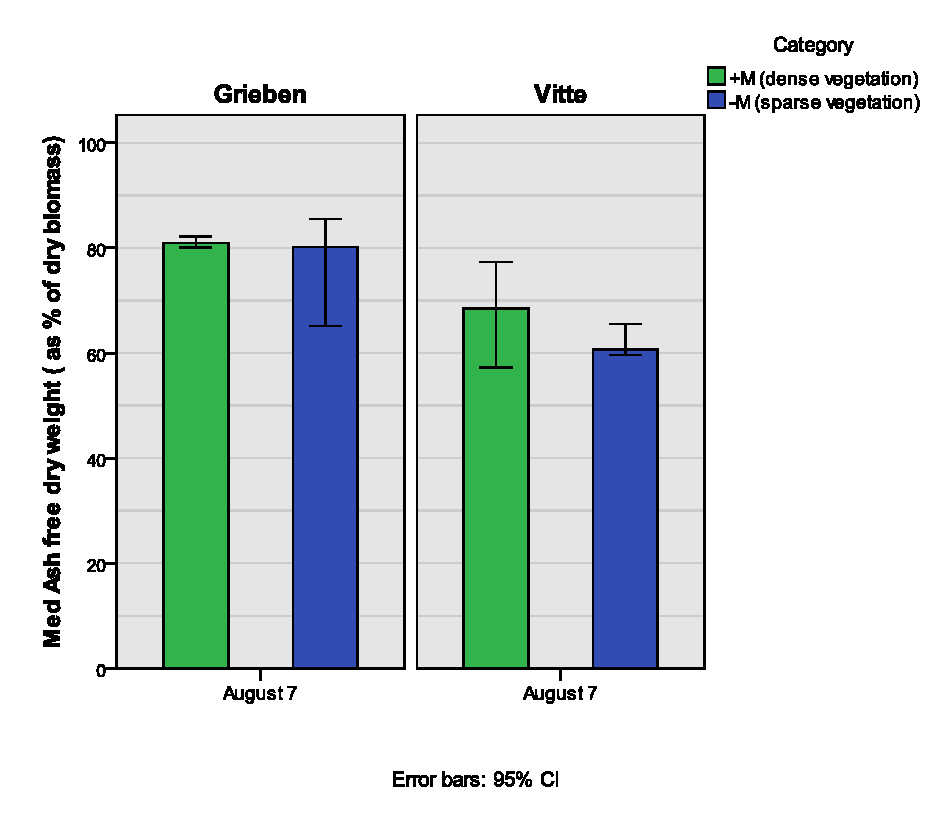
\includegraphics[width=0.80\textwidth]{images/biomass/biomasse_afdg_berichtigt1.eps}
\caption[Organischer Anteil der Biomasse an den Hiddenseer Standorten]{Organischer Anteil (ermittelt als aschfreies Trockengewicht) der Biomasse auf den Miniplots (\unit{0,25}{\metre\squared} in Grieben und Vitte, Probenahme Anfang August; Median (Balken) und \unit{95}{\%}-Bereich(Antennen) der Daten von jeweils 5 Replikaten}
\label{fig:biomasse_verascht}
\end{figure}


\FloatBarrier
\\


\begin{table}[!htb]{\textwidth}
\centering
\caption[Deskriptive Statistik, Biomasse und deren organischer Gehalt in Grieben und Vitte]{Deskriptive Statistik zur Biomasse (Dry Weight, Trockengewicht) und Organischer Gehalt (AFDW) im Vitter Bodden und in der Griebener Bucht; +M = dichte Vegetation, -M = spärliche Vegetation, MAD = Mittlere Abweichung vom Median}
\begin{tabular}{llrrrr}
\toprule
Location & Date	& \multicolumn{2}{c}{Dry Weight} 	& \multicolumn{2}{c}{AFDW}\\
&& \multicolumn{2}{c}{(\gram\per\metre\squared)} & \multicolumn{2}{c}{(\%)}\\
\midrule
							&			& Median 		& MAD				& Median		& MAD\\
\midrule
\multirow{2}{*}{Vitter Bodden (+M)}& July 	& 558.48		& 100.92			\\
 								 & August	& 890.28		& 119.74			& 68.47			& 4.77\\
\midrule
\multirow{1}{*}{Vitter Bodden (-M)}& August & 15.08			& 9.42				& 60.70			& 1.35\\
\midrule
\multirow{2}{*}{Griebener Bucht (+M)}& July & 132.12		& 30.81				\\
									& August & 126.48		& 36.50				& 80.95			& 0.62\\
\midrule	
\multirow{1}{*}{Griebener Bucht (-M)}& August & 16.52		& 9.23				& 80.16			& 5.94\\
\bottomrule
\end{tabular}
\label{tab:statistik_biomasse}
\end{table}

\FloatBarrier


\subsection{Sediment}



\begin{table}[!htb]{\textwidth}
\centering
\caption[Deskriptive Statistik, Korngrößenverteilung in Grieben und Vitte]{Deskriptive Statistik zu den Korngrößenverteilungen im Vitter Bodden (V) und in der Griebener Bucht (G); +M = dichte Vegetation, -M = spärliche Vegetation, MD = Median, MAD = Mittlere Abweichung vom Median, die Schiefe (Skewness) bezieht sich auf die Phi-Korngrößen}
\begin{tabular}{ccrrrrrrrrrr}
\toprule
Location & \multicolumn{1}{c}{Date}	& \multicolumn{2}{c}{MD Grain} 	& \multicolumn{2}{c}{Sorting} & \multicolumn{2}{c}{Skewness} & \multicolumn{2}{c}{\unit{< 63}{\mu\metre}} & \multicolumn{2}{c}{AFDW}\\
&& \multicolumn{2}{c}{Size ($ \phi $)} &&&&& \multicolumn{2}{c}{(\%)} & \multicolumn{2}{c}{(\%)}\\
\midrule
                      && MD	& MAD	& MD	&	MAD		& MD	&	MAD		& MD	&	MAD	& 	MD	&	MAD\\
\midrule
\multirow{3}{*}{V (+M)}	& Jul 05 & 2.13 & &0.54 &&&&6.04 &&1.23\\
						& Aug 01 & 2.37 & 0.03 & 0.93 & 0.07 & 0.10 & 0.05 & 9.05 & 1.79 & 1.43 & 0.41\\
						& Aug 19 & 2.08 & 0.16 & 0.93 & 0.02 & 0.22 & 0.09 & 8.61 & 0.60 & 1.70 & 0.28\\
\midrule
\multirow{3}{*}{V (-M)}	& Jul 05 & 2.69 & 	   & 0.56 &      & 	    & 	   & 5.56 &	     & 0.91\\
						& Aug 01 & 2.10 & 0.14 & 0.74 & 0.06 & 0.15 & 0.10 & 4.24 & 0.97 & 0.79 & 0.15\\
						& Aug 19 & 2.1 & 0.08 & 0.74 & 0.06 & 0.18 & 0.03 & 4.11 & 1.15 & 0.95 & 0.15\\
\midrule
\multirow{3}{*}{G (+M)}	& Jun 11 & 3.65 & 0.04 & 0.94 & 0.13 & -0.16 & 0.08 & 32.05 & 2.77 & 4.77 & 0.42\\
						& Jul 30 & 3.61 & 0.96 & 0.95 & 0.31 & -0.17 & 0.05 & 28.31 & 3.09 & 4.19 & 0.44\\
						& Aug 17 & 3.63 & 0.06 & 1.11 & 0.19 & -0.29 & 0.11 & 30.15 & 3.57 & 4.18 & 0.20\\
\midrule
\multirow{3}{*}{G (-M)} & Jun 11 & 3.47 & 0.02 & 0.66 & 0.03 & -0.09 & 0.03 & 11.95 & 1.06 & 1.69 & 0.24\\
						& Jul 30 & 3.42 & 0.11 & 0.67 & 0.04 & -0.13 & 0.08 & 10.23 & 1.30 & 1.43 & 0.06\\
						& Aug 17 & 3.47 & 0.89 & 0.66 & 0.18 & -0.09 & 0.03 & 14.38 & 4.92 & 1.65 & 0.16\\		
						
\bottomrule
\end{tabular}
\label{tab:statistik_G,V_sedimentparameter}
\end{table}





\subsubsection{Vitte, dicht bewachsener Standort}

Das Sediment auf diesen Untersuchungsflächen ändert sich nicht signifikant im Jahresverlauf in Hinsicht auf den Median der Korngrößenverteilung, die Sortierung und die Schiefe. Mit einem Anteil von \unit{40-50}{\%} beziehungsweise von \unit{30-40}{\%} dominieren die Anteile von feinem Sand (\unit{2-3}{$\phi$}) und Mittelsand (\unit{1-2}{$\phi$}). Der Median der Korngröße beträgt \unit{2,08-2,13}{$\phi$}. Das Sediment ist mäßig gut sortiert und zeigt eine positive Schiefe, das heißt, der Median der Verteilungskurve ist nach rechts in den grobkörnigeren Bereich (auf der $\phi$- Verteilungskurve nach links) verschoben. Der Anteil der \unit{< 63}{\mu\metre}-Fraktion, welche den Silt- und Tongehalt repräsentiert, beträgt im Juli \unit{6}{\%} und im August \unit{8,6-9}{\%}, die Zunahme ist jedoch nicht signifikant. Etwa gleich viel sehr feiner Sand (3-4 $\phi$) ist enthalten, während der Gehalt an Grobsanden und sehr groben Sanden vernachlässigbar ist. Der organische Gehalt des Sedimentes beträgt zwischen \unit{1,2}{\%} im Juli und \unit{1,7}{\%} Ende August. Die Zunahme des organischen Gehaltes in der Vegetationsperiode ist nicht signifikant.

\begin{figure}[!htb]
\centering
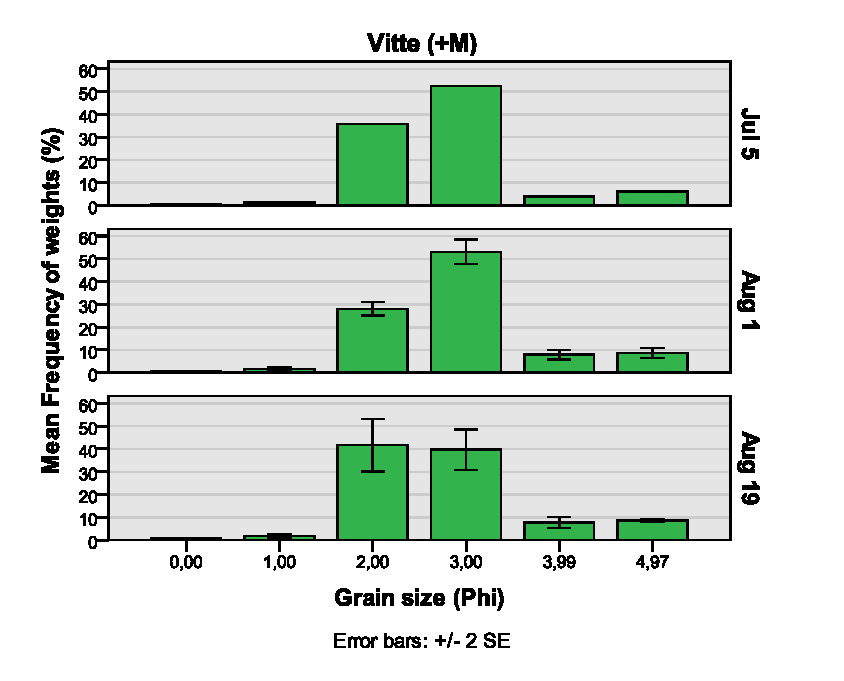
\includegraphics[width=0.70\textwidth]{images/grainsize/sediment_im_jahr1.eps}
\caption[Korngrößenverteilungen Vitte (+M)]{Korngrößenverteilungen am dicht bewachsenen Standort im Vitter Bodden; Juli: 3 Messparallelen aus einem Kern, August: Messparallelen aus 5 Sedimentkernen}
\label{fig:korngrössen_Vitte_+m}
\end{figure}



\subsubsection{Vitte, spärlich bewachsener Standort}

Die Sedimente an dieser Untersuchungsgruppe unterscheiden sich von denen auf den dicht bewachsenen Untersuchungsflächen im Vitter Bodden, jedoch mit Ausnahme des organischen Gehaltes, welcher im Mittel \unit{0,8-1}{\%} betrug. Die Verteilungskurve ist mäßig bis schlecht sortiert und ebenfalls in den grobkörnigen Bereich verschoben. Die Mittelsand und Feinsandanteile dominieren und nehmen zusammen über \unit{90}{\%} des Gesamtprobenmaterials ein. Sowohl grobe als auch sehr feine Sande sind kaum vorhanden und auch der Ton-und Silt-Anteil ist mit ca. \unit{4}{\%} etwas geringer. Das Verhältnis von Mittelsand zu Feinsand ist hier umgekehrt. Der Mittelsand hat einen größeren Anteil von etwa \unit{50}{\%} während der Feinsand einen geringeren Anteil von etwa \unit{40-45}{\%} hat. 


\begin{figure}[!htb]
\centering
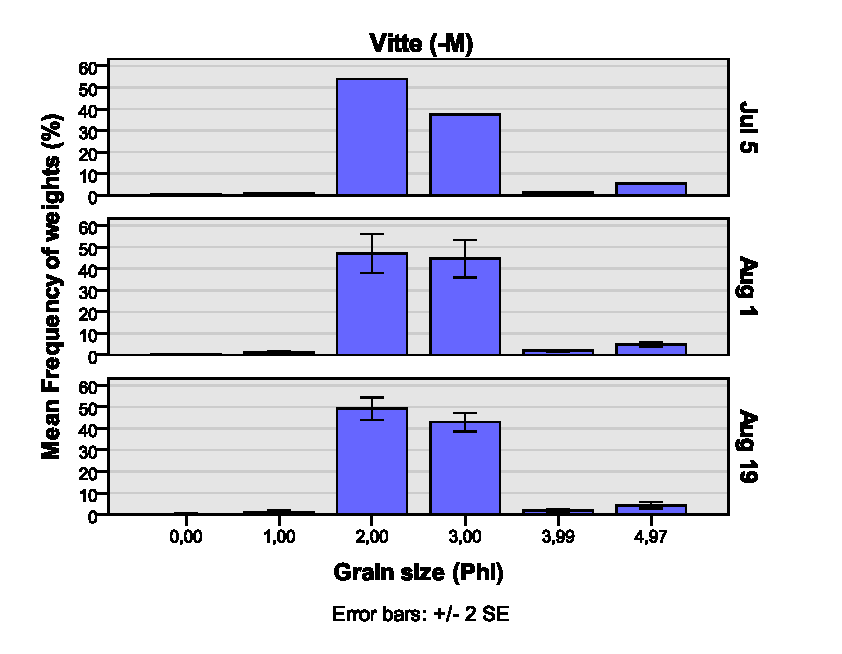
\includegraphics[width=0.70\textwidth]{images/grainsize/sediment_im_jahr2.eps}
\caption[Korngrößenverteilungen Vitte (-M)]{Korngrößenverteilungen am spärlich bewachsenen Standort im Vitter Bodden; Juli: 3 Messparallelen aus einem Kern, August: Messparallelen aus 5 Sedimentkernen}
\label{fig:korngrössen_Vitte_-m}
\end{figure}


\subsubsection{Grieben, dicht bewachsener Standort}

Die Sedimente auf den Flächen dieser Untersuchungsgruppe sind mäßig bis schlecht sortiert und zeigen eine negative Schiefe aufgrund der Dominanz der feinen Korngrößenfraktionen. Mit etwa \unit{50-52}{\%} ist sehr feiner Sand (3-4 $\phi$) am stärksten vertreten. Auch der Ton- und Siltanteil ist mit \unit{30-35}{\%} sehr hoch. Der Median der Korngröße beträgt im Mittel \unit{3,6}{$\phi$} und verringert sich zwischen Juni und Juli leicht im Jahresverlauf. Insgesamt verschiebt sich das Verteilungsmuster im Verlauf der Vegetationsperiode leicht in den feinkörnigeren Bereich. Mittelsand und Feinsand sind insgesamt mit nur etwa \unit{5 bzw 8}{\%} vertreten. Im Vergleich zu den Vitter Untersuchungsgruppen gab es eine geringe Menge (etwa \unit{2-6}{\%} sehr groben Sand beziehungsweise Kiessteinchen oder Muschelschalenreste. 
Der Organische Anteil des Sedimentes beträgt im Mittel \unit{0,2-0,4}{\%} und entspricht damit dem organischen Gehalt des vegetationsfreien Standortes im Vitter Bodden.



\begin{figure}[!htb]
\centering
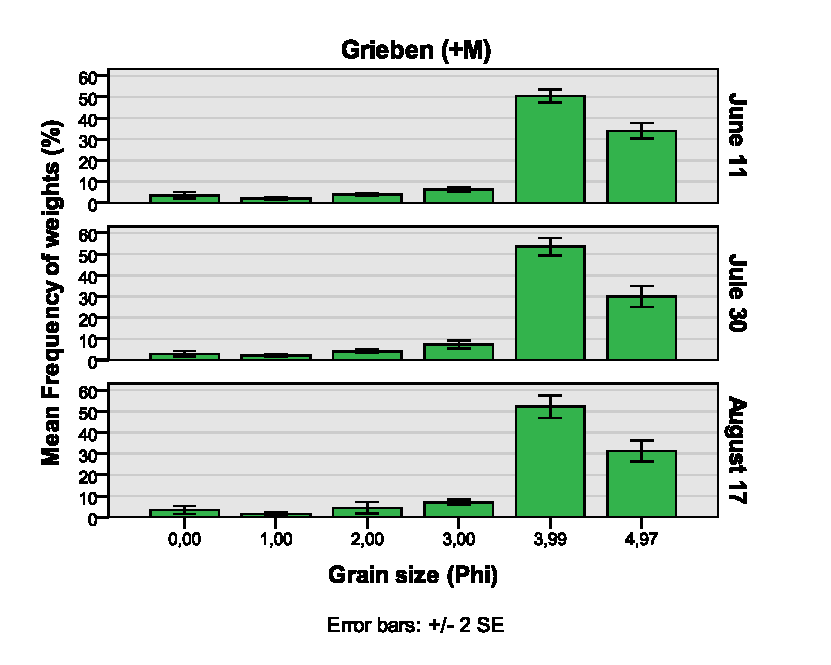
\includegraphics[width=0.70\textwidth]{images/grainsize/sediment_im_jahr3.eps}
\caption[Korngrößenverteilungen Grieben (+M)]{Korngrößenverteilungen am dicht bewachsenen Standort in der Griebener Bucht; Messparallelen aus 5 Sedimentkernen}
\label{fig:korngrössen_Grieben_+m}
\end{figure}




\subsubsection{Grieben, spärlich bewachsener Standort}

Hier ist die Korngrößenverteilung signifikant unterschiedlich gegenüber der der dicht mit Phytobenthos besiedelten Untersuchungsgruppe. Sie ist nur leicht linksschief, fast symmetrisch. Der Median der Korngröße beträgt \unit{3,42-3,47}{$\phi$}, wobei im Juli signifikant geringere Werte gefunden wurden als im Juni und im August. Das bedeutet, dass im Juli der Anteil der feinkörnigeren Fraktionen im Mittel etwas geringer war. Grund hierfür ist ein leichter Anstieg der Feinsandfraktion und ein Rückgang sehr feiner Sande, Tone und Silte. Im Mittel ist das Sediment hier etwas gröber als im dicht besiedelten Bereich der Bucht und der Silt-/ Tonanteil deutlich geringer. Grobsande sind kaum enthalten und das Sediment ist aufgrund der Dominanz der sehr feinen Sandfraktion mit einem Anteil von etwa \unit{60-70}{\%} an der Gesamtprobe mäßig sortiert. Der organische Anteil beträgt \unit{0,1-0,2}{\%} und ist deutlich geringer als am vegetationsdominierten Standort, jedoch mit dem vegetationsarmen Standort des Vitter Bodden vergleichbar.



\begin{figure}[!htb]
\centering
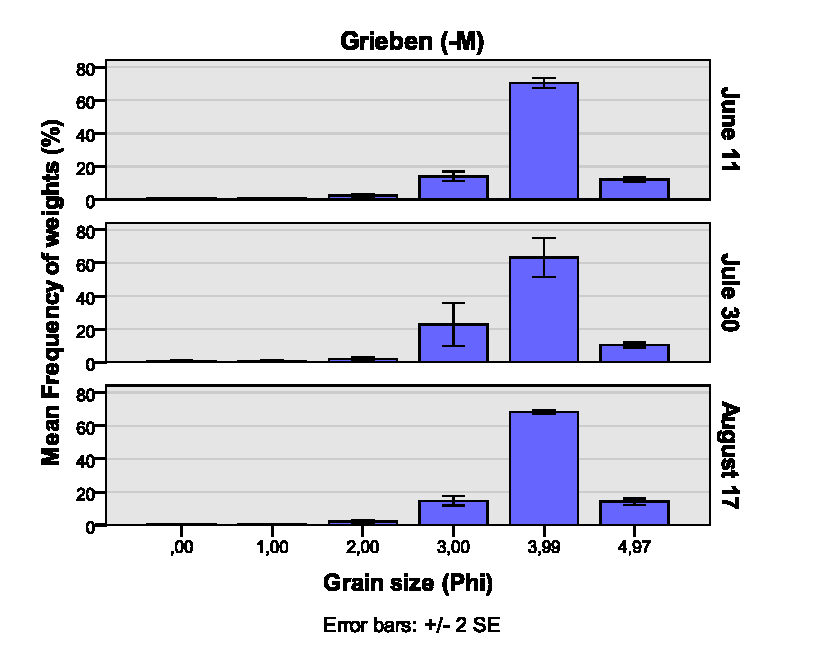
\includegraphics[width=0.70\textwidth]{images/grainsize/sediment_im_jahr4.eps}
\caption[Korngrößenverteilungen Grieben (-M)]{Korngrößenverteilungen am spärlich bewachsenen Standort in der Griebener Bucht; Messparallelen aus 5 Sedimentkernen}
\label{fig:korngrössen_Grieben_-m}
\end{figure}




\FloatBarrier



\begin{figure}[htb]
\centering
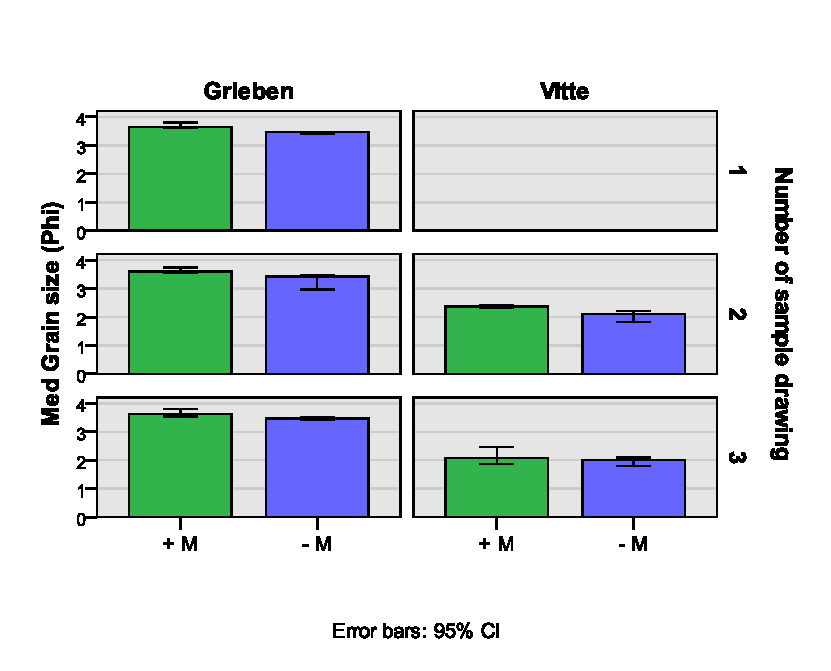
\includegraphics[width=0.70\textwidth]{images/sedimentparameter/S-Parameter_MD_KG_neu1.eps}
\caption[Median der Korngröße Grieben und Vitte]{Median der Korngröße an dicht (+M) und spärlich (-M) bewachsenen Standorten im Vitter Bodden und in der Griebener Bucht im Verlauf der Wachstumsperiode}
\label{fig:md_korngroesse_hiddensee}
\end{figure}


\begin{figure}[htb]
\centering
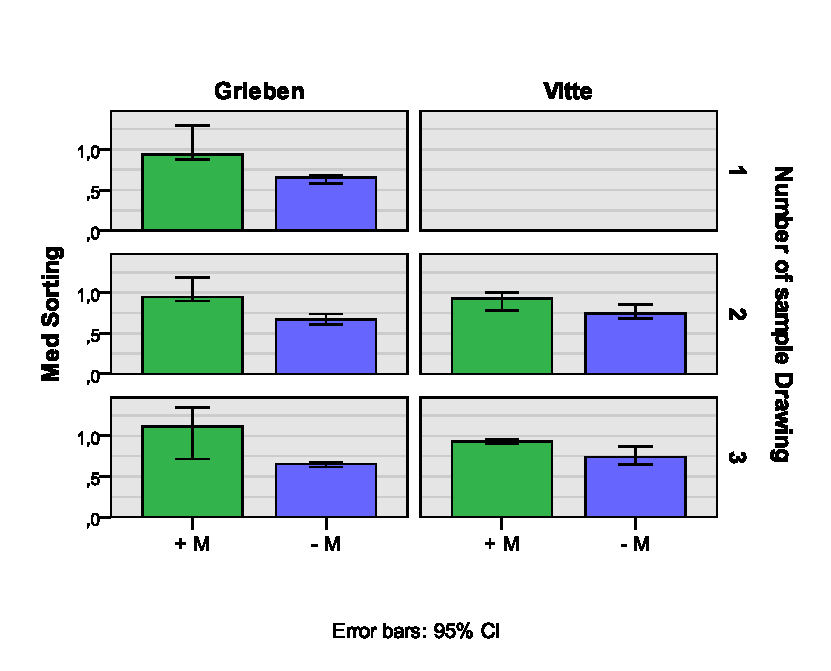
\includegraphics[width=0.70\textwidth]{images/sedimentparameter/S_Parameter_Sortierung_neu1.eps}
\caption[Sortierung der Sedimente in Grieben und Vitte]{Sortierung der Sedimente an dicht (+M) und spärlich (-M) bewachsenen Standorten im Vitter Bodden und in der Griebener Bucht im Verlauf der Wachstumsperiode}
\label{fig:sortierung}
\end{figure}



\begin{figure}[htb]
\centering
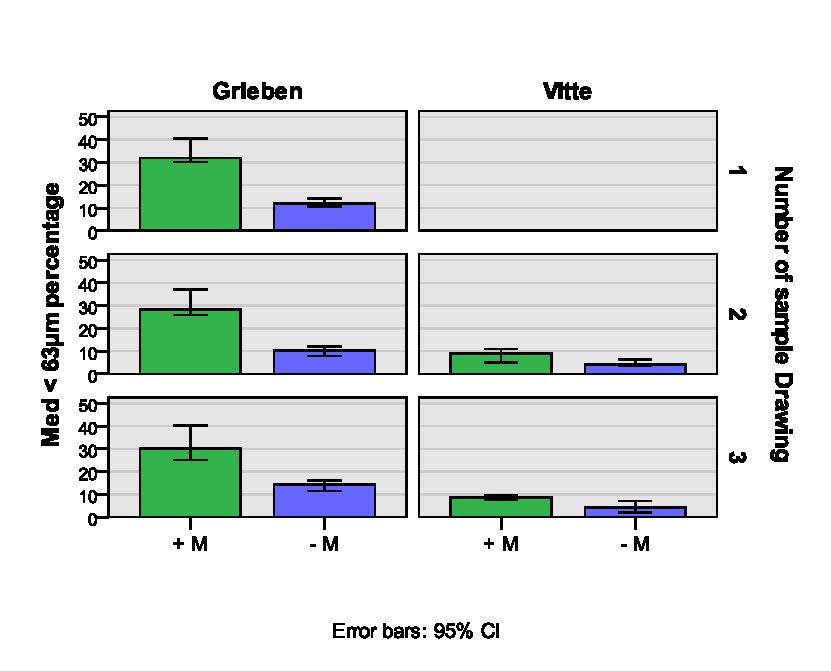
\includegraphics[width=0.70\textwidth]{images/sedimentparameter/S_Parameter_63_neu1.eps}
\caption[Anteil der \unit{<63}{\mu\metre}-Korngrößenfraktion in Grieben und Vitte]Anteil der \unit{<63}{\mu\metre}-Korngrößenfraktion an dicht (+M) und spärlich (-M) bewachsenen Standorten im Vitter Bodden und in der Griebener Bucht im Verlauf der Wachstumsperiode}
\label{fig:63}
\end{figure}


\begin{figure}[htb]
\centering
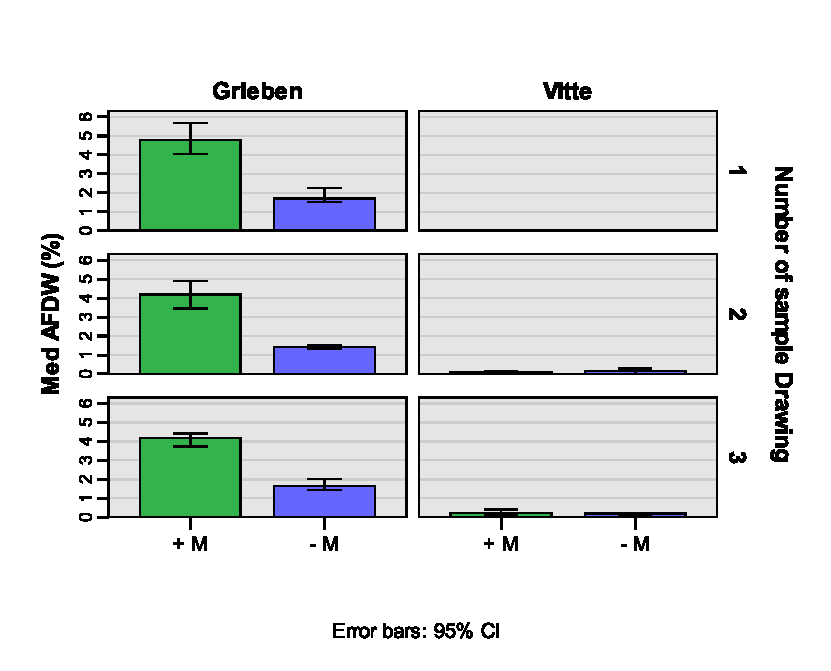
\includegraphics[width=0.70\textwidth]{images/sedimentparameter/afdg_neu1.eps}
\caption[Organischer Gehalt des Sedimentes in Grieben und Vitte]{Organischer Gehalt des Sedimentes, ermittelt als aschfreies Trockengewicht (AFDW) an dicht (+M) und spärlich (-M) bewachsenen Standorten im Vitter Bodden und in der Griebener Bucht im Verlauf der Wachstumsperiode}
\label{fig:afdg_sediment}
\end{figure}